\documentclass[11pt, dvips]{book}
\usepackage[hyperref, thmmarks]{styles/ntheorem}
\usepackage{framed}
\usepackage{times}
\usepackage{textcomp}
\usepackage{tabularx}
\usepackage{moreverb}
\usepackage[pdftex]{graphicx}
\usepackage{amssymb}
\usepackage{float}
\usepackage[dvips,
  pdftitle={JAX-RS: Java API for RESTful Web Services},
  pdfauthor={Santiago Pericas-Geertsen and Marek Potociar, Oracle},
  pdfsubject={JAX-RS: Java API for RESTful Web Services},
  pdfkeywords={Java XML Web Services API REST RESTful},
  pdftex,
  colorlinks=true,
  linkcolor=black,
  citecolor=black,
  pdfstartview=FitH,
  letterpaper=true,
  bookmarksnumbered=true
]{hyperref}

% set up page dimensions
\textwidth = 6.5 in
\textheight = 9.33 in
\oddsidemargin = 0.0 in
\evensidemargin = 0.0 in
\topmargin = -0.75 in
\headheight = 15pt
\headsep = 0.33 in
\parskip = 6pt
\parindent = 0.0in
\footskip=0.5in

\usepackage{fancyhdr}
\pagestyle{fancy}
\usepackage{styles/jsr}
\theoremstyle{plain}
%\setlength{\theorempostskipamount}{0pt}
\newtheorem{ednote}{Editors Note}[chapter]

\theoremstyle{nonumberplain}
\theoremindent0cm
\theoremseparator{:}
\newtheorem{nnnote}{Note}[chapter]

%\usepackage[pagewise, right]{styles/lineno}
%\usepackage[dvips]{changebar}
\usepackage{longtable}

%\renewcommand{\today}{September 8, 2008}

\begin{document}

\frontmatter
\newtheorem{note}{Note}[chapter]
\newcommand{\code}[1]{\texttt{\small #1}}
\renewcommand\verbatimtabsize{4\relax}
\newcommand{\jaxrs}{JAX-RS}

\newcommand{\Consumes}{\code{@Consumes}}
\newcommand{\Encoded}{\code{@Encoded}}
\newcommand{\HeaderParam}{\code{@Header\-Param}}
\newcommand{\Context}{\code{@Context}}
\newcommand{\SecurityContext}{\code{Security\-Context}}
\newcommand{\HttpHeaders}{\code{Http\-Headers}}
\newcommand{\HttpMethod}{\code{@Http\-Method}}
\newcommand{\MatrixParam}{\code{@Matrix\-Param}}
\newcommand{\MsgRead}{\code{Message\-Body\-Reader}}
\newcommand{\MsgWrite}{\code{Message\-Body\-Writer}}
\newcommand{\Path}{\code{@Path}}
\newcommand{\PathParam}{\code{@Path\-Param}}
\newcommand{\Produces}{\code{@Produces}}
\newcommand{\Provider}{\code{@Provider}}
\newcommand{\QueryParam}{\code{@Query\-Param}}
\newcommand{\FormParam}{\code{@Form\-Param}}
\newcommand{\CookieParam}{\code{@Cookie\-Param}}
\newcommand{\Request}{\code{Request}}
\newcommand{\Response}{\code{Response}}
\newcommand{\ResponseBuilder}{\code{Response\-Builder}}
\newcommand{\rd}{\code{Runtime\-Delegate}}
\newcommand{\UriInfo}{\code{Uri\-Info}}
\newcommand{\WebAppExc}{\code{Web\-Application\-Exception}}
\newcommand{\Resource}{\code{javax.\-annotation.\-Resource}}

\newcommand{\Client}{\code{Client}}
\newcommand{\ClientBuilder}{\code{ClientBuilder}}
\newcommand{\ClientConfiguration}{\code{ClientConfiguration}}
\newcommand{\Link}{\code{Link}}
\newcommand{\Invocation}{\code{Invocation}}
\newcommand{\Configurable}{\code{Configurable}}
\newcommand{\InvocationBuilder}{\code{Invocation.Builder}}

\newcommand{\ClientRequestFilter}{\code{ClientRequestFilter}}
\newcommand{\ContainerRequestFilter}{\code{ContainerRequestFilter}}
\newcommand{\ClientResponseFilter}{\code{ClientResponseFilter}}
\newcommand{\ContainerResponseFilter}{\code{ContainerResponseFilter}}
\newcommand{\PreMatching}{\code{@PreMatching}}
\newcommand{\PostMatching}{\code{@PostMatching}}
\newcommand{\ContainerRequestContext}{\code{ContainerRequestContext}}
\newcommand{\ContainerResponseContext}{\code{ContainerResponseContext}}
\newcommand{\ReaderInterceptor}{\code{ReaderInterceptor}}
\newcommand{\WriterInterceptor}{\code{WriterInterceptor}}
\newcommand{\ReaderInterceptorContext}{\code{ReaderInterceptorContext}}
\newcommand{\WriterInterceptorContext}{\code{WriterInterceptorContext}}
\newcommand{\MessageBodyReader}{\code{MessageBodyReader}}
\newcommand{\MessageBodyWriter}{\code{MessageBodyWriter}}
\newcommand{\DynamicBinder}{\code{DynamicBinder}}
\newcommand{\DynamicFeature}{\code{DynamicFeature}}
\newcommand{\ParamConverter}{\code{ParamConverter}}
\newcommand{\ParamConverterProvider}{\code{ParamConverterProvider}}

\newcommand{\NameBinding}{\code{@NameBinding}}
\newcommand{\GlobalBinding}{\code{@GlobalBinding}}
\newcommand{\Priority}{\code{@Priority}}

\newcommand{\NotNull}{\code{@NotNull}}
\newcommand{\ApplicationPath}{\code{@ApplicationPath}}
\newcommand{\Email}{\code{@Email}}
\newcommand{\Pattern}[1]{\code{@Pattern(#1)}}
\newcommand{\Constraint}{\code{@Constraint}}
\newcommand{\Valid}{\code{@Valid}}
\newcommand{\Suspended}{\code{@Suspended}}
\newcommand{\ExecutionContext}{\code{ExecutionContext}}
\newcommand{\WebApplicationException}{\code{WebApplicationException}}
\newcommand{\WebTarget}{\code{WebTarget}}

\newcommand{\ClientRequest}{{\footnotesize {\sf ClientRequest}}}
\newcommand{\ClientResponse}{{\footnotesize {\sf ClientResponse}}}
\newcommand{\ContainerRequest}{{\footnotesize {\sf ContainerRequest}}}
\newcommand{\PreMatchContainerRequest}{{\footnotesize {\sf PreMatchContainerRequest}}}
\newcommand{\ContainerResponse}{{\footnotesize {\sf ContainerResponse}}}
\newcommand{\ReadFrom}{{\footnotesize {\sf ReadFrom}}}
\newcommand{\WriteTo}{{\footnotesize {\sf WriteTo}}}


% set up page styles for frontmatter, no page headers, normal footer
\fancyhf{}
\fancyfoot[CO,CE]{JAX-RS}
\fancyfoot[LE,RO]{\thepage}
\fancyfoot[RE,LO]{\today} 
\fancypagestyle{plain}{
  \fancyhf{}
  \fancyfoot[CO,CE]{JAX-RS}
  \fancyfoot[LE,RO]{\thepage}
  \fancyfoot[RE,LO]{\today} 
  \renewcommand{\footrulewidth}{0pt}
  \renewcommand{\headrulewidth}{0pt}
}
\renewcommand{\headrulewidth}{0pt}


\begin{titlepage}
\raggedleft

\vspace*{60pt}

{\Huge
\textsf{JAX-RS: Java\texttrademark\ API for RESTful\\\vspace{10pt}
 Web Services}}

\vspace{20pt}

{
\Large\textit{Version 2.0 Final Release\\
\today}
}

\vspace{40pt}

{\large Editors:\\
Santiago\ Pericas-Geertsen\\
Marek\ Potociar\\
\vspace{10pt}Comments to: users@jax-rs-spec.java.net
}

\vspace{80pt}

{\small\textit{Oracle Corporation\\
500 Oracle Parkway, Redwood Shores, CA 94065 USA.}
}
\end{titlepage} 


\cleardoublepage
{
\small
\begin{flushleft}

{\bfseries JSR-339 Java\texttrademark\ API for RESTful Web Services (\lq\lq Specification\rq\rq)\\
Version: 2.0 \\
Status: Final Release \\
Release: \today\\ 
Copyright 2011-2013 Oracle America, Inc. (``Oracle'') \\
500 Oracle Parkway, Redwood Shores, California 94065, U.S.A\\ 
All rights reserved.
}

\mbox{}\\
{\bfseries LIMITED LICENSE GRANTS}

1. License for Evaluation Purposes. Oracle hereby grants you a fully-paid, non-exclusive, non-transferable, worldwide, limited license (without the right to sublicense), under Oracle's  applicable intellectual property rights to view, download, use and reproduce the Specification only for the purpose of internal evaluation.  This includes (i) developing applications intended to run on an implementation of the Specification, provided that such applications do not themselves implement any portion(s) of the Specification, and (ii) discussing the Specification with any third party; and (iii) excerpting brief portions of the Specification in oral or written communications which discuss the Specification provided that such excerpts do not in the aggregate constitute a significant portion of the Specification.

2. License for the Distribution of Compliant Implementations. Oracle  also grants you a perpetual, non-exclusive, non-transferable, worldwide, fully paid-up, royalty free, limited license (without the right to sublicense) under any applicable copyrights or, subject to the provisions of subsection 4 below, patent rights it may have covering the Specification to create and/or distribute an Independent Implementation of the Specification that: (a) fully implements the Specification including all its required interfaces and functionality; (b) does not modify, subset, superset or otherwise extend the Licensor Name Space, or include any public or protected packages, classes, Java interfaces, fields or methods within the Licensor Name Space other than those required/authorized by the Specification or Specifications being implemented; and (c) passes the Technology Compatibility Kit (including satisfying the requirements of the applicable TCK Users Guide) for such Specification ("Compliant Implementation").  In addition, the foregoing license is expressly conditioned on your not acting outside its scope.  No license is granted hereunder for any other purpose (including, for example, modifying the Specification, other than to the extent of your fair use rights, or distributing the Specification to third parties).  Also, no right, title, or interest in or to any trademarks, service marks, or trade names of Oracle or Oracle's licensors is granted hereunder.  Java, and Java-related logos, marks and names are trademarks or registered trademarks of Oracle America, Inc. in the U.S. and other countries.

3. Pass-through Conditions. You need not include limitations (a)-(c) from the previous paragraph or any other particular "pass through" requirements in any license You grant concerning the use of your Independent Implementation or products derived from it.  However, except with respect to Independent Implementations (and products derived from them) that satisfy limitations (a)-(c) from the previous paragraph, You may neither:  (a) grant or otherwise pass through to your licensees any licenses under Oracle’s applicable intellectual property rights; nor (b) authorize your licensees to make any claims concerning their implementation's compliance with the Specification in question.

4. Reciprocity Concerning Patent Licenses.  

 \hspace{1em} a. With respect to any patent claims covered by the license granted under subparagraph 2 above that would be infringed by all technically feasible implementations of the Specification, such license is conditioned upon your offering on fair, reasonable and non-discriminatory terms, to any party seeking it from You, a perpetual, non-exclusive, non-transferable, worldwide license under Your patent rights which are or would be infringed by all technically feasible implementations of the Specification to develop, distribute and use a Compliant Implementation.

 \hspace{1em} b. With respect to any patent claims owned by Oracle and covered by the license granted under subparagraph 2, whether or not their infringement can be avoided in a technically feasible manner when implementing the Specification, such license shall terminate with respect to such claims if You initiate a claim against Oracle that it has, in the course of performing its responsibilities as the Specification Lead, induced any other entity to infringe Your patent rights.

 \hspace{1em} c. Also with respect to any patent claims owned by Oracle and covered by the license granted under subparagraph 2 above, where the infringement of such claims can be avoided in a technically feasible manner when implementing the Specification such license, with respect to such claims, shall terminate if You initiate a claim against Oracle  that its making, having made, using, offering to sell, selling or importing a Compliant Implementation infringes Your patent rights.

5. Definitions. For the purposes of this Agreement:  "Independent Implementation" shall mean an implementation of the Specification that neither derives from any of Oracle's  source code or binary code materials nor, except with an appropriate and separate license from Oracle, includes any of Oracle's  source code or binary code materials; "Licensor Name Space" shall mean the public class or interface declarations whose names begin with "java", "javax", "com.sun", “com.oracle”  or their equivalents in any subsequent naming convention adopted by Oracle  through the Java Community Process, or any recognized successors or replacements thereof; and "Technology Compatibility Kit" or "TCK" shall mean the test suite and accompanying TCK User's Guide provided by Oracle  which corresponds to the Specification and that was available either (i) from Oracle 120 days before the first release of Your Independent Implementation that allows its use for commercial purposes, or (ii) more recently than 120 days from such release but against which You elect to test Your implementation of the Specification.

This Agreement will terminate immediately without notice from Oracle if you breach the Agreement or act outside the scope of the licenses granted above.

{\bfseries DISCLAIMER OF WARRANTIES}

THE SPECIFICATION IS PROVIDED "AS IS". ORACLE MAKES NO REPRESENTATIONS OR WARRANTIES, EITHER EXPRESS OR IMPLIED, INCLUDING BUT NOT LIMITED TO, WARRANTIES OF MERCHANTABILITY, FITNESS FOR A PARTICULAR PURPOSE, NON-INFRINGEMENT (INCLUDING AS A CONSEQUENCE OF ANY PRACTICE OR IMPLEMENTATION OF THE SPECIFICATION), OR THAT THE CONTENTS OF THE SPECIFICATION ARE SUITABLE FOR ANY PURPOSE.  This document does not represent any commitment to release or implement any portion of the Specification in any product. In addition, the Specification could include technical inaccuracies or typographical errors.

{\bfseries LIMITATION OF LIABILITY}

TO THE EXTENT NOT PROHIBITED BY LAW, IN NO EVENT WILL ORACLE OR ITS LICENSORS BE LIABLE FOR ANY DAMAGES, INCLUDING WITHOUT LIMITATION, LOST REVENUE, PROFITS OR DATA, OR FOR SPECIAL, INDIRECT, CONSEQUENTIAL, INCIDENTAL OR PUNITIVE DAMAGES, HOWEVER CAUSED AND REGARDLESS OF THE THEORY OF LIABILITY, ARISING OUT OF OR RELATED IN ANY WAY TO YOUR HAVING, IMPLEMENTING OR OTHERWISE USING  THE SPECIFICATION, EVEN IF ORACLE AND/OR ITS LICENSORS HAVE BEEN ADVISED OF THE POSSIBILITY OF SUCH DAMAGES. 
You will indemnify, hold harmless, and defend Oracle and its licensors from any claims arising or resulting from: (i) your use of the Specification; (ii) the use or distribution of your Java application, applet and/or implementation; and/or (iii) any claims that later versions or releases of any Specification furnished to you are incompatible with the Specification provided to you under this license. 

{\bfseries RESTRICTED RIGHTS LEGEND}

U.S. Government: If this Specification is being acquired by or on behalf of the U.S. Government or by a U.S. Government prime contractor or subcontractor (at any tier), then the Government's rights in the Software and accompanying documentation shall be only as set forth in this license; this is in accordance with 48 C.F.R. 227.7201 through 227.7202-4 (for Department of Defense (DoD) acquisitions) and with 48 C.F.R. 2.101 and 12.212 (for non-DoD acquisitions). 

{\bfseries REPORT}

If you provide Oracle with any comments or suggestions concerning the Specification ("Feedback"), you hereby: (i) agree that such Feedback is provided on a non-proprietary and non-confidential basis, and (ii) grant Oracle a perpetual, non-exclusive, worldwide, fully paid-up, irrevocable license, with the right to sublicense through multiple levels of sublicensees, to incorporate, disclose, and use without limitation the Feedback for any purpose.

{\bfseries GENERAL TERMS}

Any action related to this Agreement will be governed by California law and controlling U.S. federal law. The U.N. Convention for the International Sale of Goods and the choice of law rules of any jurisdiction will not apply.

The Specification is subject to U.S. export control laws and may be subject to export or import regulations in other countries. Licensee agrees to comply strictly with all such laws and regulations and acknowledges that it has the responsibility to obtain such licenses to export, re-export or import as may be required after delivery to Licensee.

This Agreement is the parties' entire agreement relating to its subject matter. It supersedes all prior or contemporaneous oral or written communications, proposals, conditions, representations and warranties and prevails over any conflicting or additional terms of any quote, order,  acknowledgment, or other communication between the parties relating to its subject matter during the term of this Agreement. No modification to this Agreement will be binding, unless in writing and signed by an authorized representative of each party.

Rev. December, 2010

\end{flushleft}

%\begin{flushleft}

{\bfseries Specification: JSR-000311 - Java\texttrademark\ API for RESTful Web Services (\lq\lq Specification\rq\rq)\\
Version: 1.1\\
Status: Final Release\\
Release: \today\\
Copyright 2007 Sun Microsystems, Inc.\\
4150 Network Circle, Santa Clara, California 95054, U.S.A\\
180, Avenue de L'Europe, 38330 Montbonnot Saint Martin, France\\
All rights reserved.
}

{\bfseries LIMITED LICENSE GRANTS}

\begin{enumerate}
\item License for Evaluation Purposes. Sun hereby grants you a fully-paid, non-exclusive, non-transferable, worldwide, limited license (without the right to sublicense), under Sun's �applicable intellectual property rights to view, download, use and reproduce the Specification only for the purpose of internal evaluation. �This includes (i) developing applications intended to run on an implementation of the Specification, provided that such applications do not themselves implement any portion(s) of the Specification, and (ii) discussing the Specification with any third party; and (iii) excerpting brief portions of the Specification in oral or written communications which discuss the Specification provided that such excerpts do not in the aggregate constitute a significant portion of the Specification.

\item License for the Distribution of Compliant Implementations. Sun �also grants you a perpetual, non-exclusive, non-transferable, worldwide, fully paid-up, royalty free, limited license (without the right to sublicense) under any applicable copyrights or, subject to the provisions of subsection 4 below, patent rights it may have covering the Specification to create and/or distribute an Independent Implementation of the Specification that: (a) fully implements the Specification including all its required interfaces and functionality; (b) does not modify, subset, superset or otherwise extend the Licensor Name Space, or include any public or protected packages, classes, Java interfaces, fields or methods within the Licensor Name Space other than those required/authorized by the Specification or Specifications being implemented; and (c) passes the Technology Compatibility Kit (including satisfying the requirements of the applicable TCK Users Guide) for such Specification (\lq\lq Compliant Implementation\rq\rq). �In addition, the foregoing license is expressly conditioned on your not acting outside its scope. �No license is granted hereunder for any other purpose (including, for example, modifying the Specification, other than to the extent of your fair use rights, or distributing the Specification to third parties). �Also, no right, title, or interest in or to any trademarks, service marks, or trade names of Sun or Sun's licensors is granted hereunder. �Java, and Java-related logos, marks and names are trademarks or registered trademarks of Sun Microsystems, Inc. in the U.S. and other countries.

\item Pass-through Conditions. You need not include limitations (a)-(c) from the previous paragraph or any other particular \lq\lq pass through\rq\rq\ requirements in any license You grant concerning the use of your Independent Implementation or products derived from it. �However, except with respect to Independent Implementations (and products derived from them) that satisfy limitations (a)-(c) from the previous paragraph, You may neither: �(a) grant or otherwise pass through to your licensees any licenses under Sun's �applicable intellectual property rights; nor (b) authorize your licensees to make any claims concerning their implementation's compliance with the Specification in question.

\item Reciprocity Concerning Patent Licenses. �
\begin{enumerate}
\item�With respect to any patent claims covered by the license granted under subparagraph 2 above that would be infringed by all technically feasible implementations of the Specification, such license is conditioned upon your offering on fair, reasonable and non-discriminatory terms, to any party seeking it from You, a perpetual, non-exclusive, non-transferable, worldwide license under Your patent rights which are or would be infringed by all technically feasible implementations of the Specification to develop, distribute and use a Compliant Implementation.

\item�With respect to any patent claims owned by Sun and covered by the license granted under subparagraph 2, whether or not their infringement can be avoided in a technically feasible manner when implementing the Specification, such license shall terminate with respect to such claims if You initiate a claim against Sun that it has, in the course of performing its responsibilities as the Specification Lead, induced any other entity to infringe Your patent rights.

\item�Also with respect to any patent claims owned by Sun and covered by the license granted under subparagraph 2 above, where the infringement of such claims can be avoided in a technically feasible manner when implementing the Specification such license, with respect to such claims, shall terminate if You initiate a claim against Sun �that its making, having made, using, offering to sell, selling or importing a Compliant Implementation infringes Your patent rights.
\end{enumerate}

\item Definitions. For the purposes of this Agreement: �\lq\lq Independent 
Implementation\rq\rq\ shall mean an implementation of the Specification that 
neither derives from any of Sun's �source code or binary code materials nor, 
except with an appropriate and separate license from Sun, includes any of Sun's 
source code or binary code materials; \lq\lq Licensor Name Space\rq\rq\ shall 
mean the public class or interface declarations whose names begin with \lq\lq 
java\rq\rq, \lq\lq javax\rq\rq, \lq\lq com.sun\rq\rq\ or their equivalents in 
any subsequent naming convention adopted by Sun �through the Java Community 
Process, or any recognized successors or replacements thereof; and \lq\lq 
Technology Compatibility Kit\rq\rq\ or \lq\lq TCK\rq\rq\ shall mean the test 
suite and accompanying TCK User's Guide provided by Sun �which corresponds to 
the Specification and that was available either (i) from Sun's 120 days before 
the first release of Your Independent Implementation that allows its use for 
commercial purposes, or (ii) more recently than 120 days from such release but 
against which You elect to test Your implementation of the Specification.
\end{enumerate}

This Agreement will terminate immediately without notice from Sun if you breach the Agreement or act outside the scope of the licenses granted above.

{\bfseries TRADEMARKS}

No right, title, or interest in or to any trademarks, service marks, or trade names of Sun or Sun's licensors is granted hereunder.  Sun, Sun Microsystems, the Sun logo, Java,  are trademarks or registered trademarks of Sun Microsystems, Inc. in the
U.S. and other countries.

{\bfseries DISCLAIMER OF WARRANTIES}

THE SPECIFICATION IS PROVIDED \lq\lq AS IS\rq\rq. SUN MAKES NO REPRESENTATIONS OR WARRANTIES, EITHER EXPRESS OR IMPLIED, INCLUDING BUT NOT LIMITED TO, WARRANTIES OF MERCHANTABILITY, FITNESS FOR A PARTICULAR PURPOSE, NON-INFRINGEMENT (INCLUDING AS A CONSEQUENCE OF ANY PRACTICE OR IMPLEMENTATION OF THE SPECIFICATION), OR THAT THE CONTENTS OF THE SPECIFICATION ARE SUITABLE FOR ANY PURPOSE. �This document does not represent any commitment to release or implement any portion of the Specification in any product. In addition, the Specification could include technical inaccuracies or typographical errors.

{\bfseries LIMITATION OF LIABILITY}

TO THE EXTENT NOT PROHIBITED BY LAW, IN NO EVENT WILL SUN OR ITS LICENSORS BE LIABLE FOR ANY DAMAGES, INCLUDING WITHOUT LIMITATION, LOST REVENUE, PROFITS OR DATA, OR FOR SPECIAL, INDIRECT, CONSEQUENTIAL, INCIDENTAL OR PUNITIVE DAMAGES, HOWEVER CAUSED AND REGARDLESS OF THE THEORY OF LIABILITY, ARISING OUT OF OR RELATED IN ANY WAY TO YOUR HAVING, IMPELEMENTING OR OTHERWISE USING USING �THE SPECIFICATION, EVEN IF SUN AND/OR ITS LICENSORS HAVE BEEN ADVISED OF THE POSSIBILITY OF SUCH DAMAGES.

You will indemnify, hold harmless, and defend Sun and its licensors from any claims arising or resulting from: (i) your use of the Specification; (ii) the use or distribution of your Java application, applet and/or implementation; and/or (iii) any claims that later versions or releases of any Specification furnished to you are incompatible with the Specification provided to you under this license. 

{\bfseries RESTRICTED RIGHTS LEGEND}

U.S. Government: If this Specification is being acquired by or on behalf of the U.S. Government or by a U.S. Government prime contractor or subcontractor (at any tier), then the Government's rights in the Software and accompanying documentation shall be only as set forth in this license; this is in accordance with 48 C.F.R. 227.7201 through 227.7202-4 (for Department of Defense (DoD) acquisitions) and with 48 C.F.R. 2.101 and 12.212 (for non-DoD acquisitions).

{\bfseries REPORT}

If you provide Sun with any comments or suggestions concerning the Specification (\lq\lq Feedback\rq\rq), you hereby: (i) agree that such Feedback is provided on a non-proprietary and non-confidential basis, and (ii) grant Sun a perpetual, non-exclusive, worldwide, fully paid-up, irrevocable license, with the right to sublicense through multiple levels of sublicensees, to incorporate, disclose, and use without limitation the Feedback for any purpose.

{\bfseries GENERAL TERMS}

Any action related to this Agreement will be governed by California law and controlling U.S. federal law. The U.N. Convention for the International Sale of Goods and the choice of law rules of any jurisdiction will not apply.

The Specification is subject to U.S. export control laws and may be subject to export or import regulations in other countries. Licensee agrees to comply strictly with all such laws and regulations and acknowledges that it has the responsibility to obtain such licenses to export, re-export or import as may be required after delivery to Licensee.

This Agreement is the parties' entire agreement relating to its subject matter. It supersedes all prior or contemporaneous oral or written communications, proposals, conditions, representations and warranties and prevails over any conflicting or additional terms of any quote, order, �acknowledgment, or other communication between the parties relating to its subject matter during the term of this Agreement. No modification to this Agreement will be binding, unless in writing and signed by an authorized representative of each party.

Rev. April, 2006
\end{flushleft}
}

\pdfbookmark[0]{Contents}{toc}
\tableofcontents

\mainmatter
% set up page styles for mainmatter, page headers and normal footer
\renewcommand{\chaptermark}[1]{
  \markboth{\chaptername
  \ \thechapter.\ #1}{}}
\renewcommand{\sectionmark}[1]{
  \markright{\thesection.\ #1}{}}
\fancyhf{}
\fancyhead[RO]{\slshape \rightmark}
\fancyhead[LE]{\slshape \leftmark}
\fancyfoot[CO,CE]{JAX-RS}
\fancyfoot[LE,RO]{\thepage}
\fancyfoot[RE,LO]{\today} 
\fancypagestyle{plain}{
  \fancyhf{}
  \fancyfoot[CO,CE]{JAX-RS}
  \fancyfoot[LE,RO]{\thepage}
  \fancyfoot[RE,LO]{\today} 
  \renewcommand{\footrulewidth}{0pt}
  \renewcommand{\headrulewidth}{0pt}
}
\renewcommand{\headrulewidth}{0.4pt}


%\linenumbers
%\nochangebars

\setcounter{secnumdepth}{4}

\newcommand{\footnoteremember}[2]{\footnote{#2}\newcounter{#1}\setcounter{#1}{\value{footnote}}}
\newcommand{\footnoterecall}[1]{\footnotemark[\value{#1}]}

\chapter{Introduction}

This specification defines a set of Java APIs for the development of Web services built according to the Representational State Transfer\cite{rest} (REST) architectural style. Readers are assumed to be familiar with 
REST; for more information about the REST architectural style and RESTful Web services, see:

\begin{itemize}
\item Architectural Styles and the Design of Network-based Software Architectures\cite{rest}
\item The REST Wiki\cite{restwiki}
\item Representational State Transfer on Wikipedia\cite{restwikipedia}
\end{itemize}

\section{Status}
\label{status}

%This is an early draft; this specification is not yet complete. A list of open issues can %be found at:
%This is a JCP public review draft; this specification is not yet final. A list of open issues can be found at:
%This is a JCP final specification. A list of open issues can be found at:

This is the final release of version 2.0. The issue tracking system for this release can be found at:

\begin{quote}
http://java.net/jira/browse/JAX\_RS\_SPEC
\end{quote}

The corresponding Javadocs can be found online at:

\begin{quote}
http://jax-rs-spec.java.net/
\end{quote}

The reference implementation can be obtained from:

\begin{quote}
http://jersey.java.net/
\end{quote}

The expert group seeks feedback from the community on any aspect of this specification, please send comments to:

\begin{quote}
users@jax-rs-spec.java.net
\end{quote}

\section{Goals}

The following are the goals of the API:

\begin{description}

\item[POJO-based] The API will provide a set of annotations and associated classes/interfaces that may be used with POJOs in order to expose them as Web resources. The specification will define object lifecycle and scope.

\item[HTTP-centric] The specification will assume HTTP\cite{http11} is the underlying network protocol and will provide a clear mapping between HTTP and URI\cite{uri} elements and the corresponding API classes and annotations. The API will provide high level support for common HTTP usage patterns and will be sufficiently flexible to support a variety of HTTP applications including WebDAV\cite{webdav} and the Atom Publishing Protocol\cite{atompub}.

\item[Format independence] The API will be applicable to a wide variety of HTTP entity body content types. It will provide the necessary pluggability to allow additional types to be added by an application in a standard manner.

\item[Container independence] Artifacts using the API will be deployable in a variety of Web-tier containers. The specification will define how artifacts are deployed in a Servlet\cite{servlet} container and as a JAX-WS\cite{jsr224} Provider.

\item[Inclusion in Java EE] The specification will define the environment for a Web resource class hosted in a Java EE container and will specify how to use Java EE features and components within a Web resource class.

\end{description}

\section{Non-Goals}
\label{non_goals}

The following are non-goals:

\begin{description}

\item[Support for Java versions prior to J2SE 6.0] The API will make extensive use of annotations and will require J2SE 6.0 or later.

\item[Description, registration and discovery] The specification will neither define nor require any service description, registration or discovery capability.

\item[HTTP Stack] The specification will not define a new HTTP stack. HTTP protocol support is provided by a container that hosts artifacts developed using the API.

\item[Data model/format classes] The API will not define classes that support manipulation of entity body content, rather it will provide pluggability to allow such classes to be used by artifacts developed using the API.

\end{description}

\section{Conventions}

The keywords `MUST', `MUST NOT', `REQUIRED', `SHALL', `SHALL NOT', `SHOULD', `SHOULD NOT', `RECOMMENDED', `MAY', and `OPTIONAL' in this document are to be interpreted as described in RFC 2119\cite{rfc2119}. 

Java code and sample data fragments are formatted as shown in figure \ref{ex1}:

\begin{figure}[hbtp]
\caption{Example Java Code}
\label{ex1}
\begin{listing}{1}
package com.example.hello;

public class Hello {
    public static void main(String args[]) {
        System.out.println("Hello World");
    }
}\end{listing}
\end{figure}

URIs of the general form `http://example.org/...' and `http://example.com/...' represent application or context-dependent URIs.

All parts of this specification are normative, with the exception of examples, notes and sections explicitly marked as `Non-Normative'. Non-normative notes are formatted as shown below.

\begin{nnnote*}
This is a note.
\end{nnnote*}

\section{Terminology}
\label{terminology}

\begin{description}
\item[Resource class] A Java class that uses \jaxrs\ annotations to implement a corresponding Web resource, see Chapter \ref{resources}.
\item[Root resource class] A {\em resource class} annotated with \Path. Root resource classes provide the roots of the resource class tree and provide access to sub-resources, see Chapter \ref{resources}.
\item[Request method designator] A runtime annotation annotated with \HttpMethod. Used to identify the HTTP request method to be handled by a {\em resource method}.
\item[Resource method] A method of a {\em resource class} annotated with a {\em request method designator} that is used to handle requests on the corresponding resource, see Section \ref{resource_method}.
\item[Sub-resource locator] A method of a {\em resource class} that is used to locate sub-resources of the corresponding resource, see Section \ref{sub_resources}.
\item[Sub-resource method] A method of a {\em resource class} that is used to handle requests on a sub-resource of the corresponding resource, see Section \ref{sub_resources}.
\item[Provider] An implementation of a \jaxrs\ extension interface. Providers extend the capabilities of a \jaxrs\ runtime and are described in Chapter \ref{providers}.
\item[Filter] A provider used for filtering request and responses.
\item[Entity Interceptor] A provider used for intercepting calls to message body readers and writers.
\item[Invocation] A Client API object that can be configured to issue an HTTP request.
\item[WebTarget] The recipient of an Invocation, identified by a URI.
\item[Link] A URI with additional meta-data such as a media type, a relation, a title, etc.

\end{description}

\section{Expert Group Members} 
\label{expert_group}

This specification is being developed as part of JSR 339 under the Java Community Process. It is the result of the collaborative work of the members of the JSR 339 Expert Group. The following are the present expert group members:

\begin{list}{$-$}{\parsep 0em \labelwidth 0em}
\item Jan Algermissen (Individual Member)
\item Florent Benoit (OW2)
\item Sergey Beryozkin (Talend) 
\item Adam Bien (Individual Member) 
\item Bill Burke (Red Hat Middleware LLC) 
\item Clinton Combs (Individual Member) 
\item Bill De Hora (Individual Member)  
\item Markus Karg (Individual Member) 
\item Sastri Malladi (Ebay) 
\item Wendy Raschke (IBM)
\item Julian Reschke (Individual Member)
\item Guilherme Silveira (Individual Member) 
\item Dionysios Synodinos (Individual Member)
\end{list}

The following are former group members of the JSR 339 Expert Group:

\begin{list}{$-$}{\parsep 0em \labelwidth 0em}
\item Tony Ng (Ebay)
\end{list}

JAX-RS 1.X has been developed as part of JSR 311 under the Java Community Process. The following were group members of the JSR 311 Expert Group:

\begin{list}{$-$}{\parsep 0em \labelwidth 0em}
\item Heiko Braun (Red Hat Middleware LLC) 
\item Larry Cable (BEA Systems)
\item Roy Fielding (Day Software, Inc.)
\item Harpreet Geekee (Nortel)
\item Nickolas Grabovas (Individual Member)
\item Mark Hansen (Individual Member)
\item John Harby (Individual Member)
\item Hao He (Individual Member)
\item Ryan Heaton (Individual Member)
\item David Hensley (Individual Member) 
\item Stephan Koops (Individual Member)
\item Changshin Lee (NCsoft Corporation) 
\item Francois Leygues (Alcatel-Lucent) 
\item Jerome Louvel (Individual Member) 
\item Hamid Ben Malek (Fujitsu Limited) 
\item Ryan J. McDonough (Individual Member) 
\item Felix Meschberger (Day Software, Inc.) 
\item David Orchard (BEA Systems) 
\item Dhanji R. Prasanna (Individual Member) 
\item Julian Reschke (Individual Member) 
\item Jan Schulz-Hofen (Individual Member) 
\item Joel Smith (IBM) 
\item Stefan Tilkov (innoQ Deutschland GmbH)
\end{list}

\section{Acknowledgements}
\label{acks}

During the course of this JSR we received many excellent suggestions. Special thanks to Martin Matula, Gerard Davison, Jakub Podlesak and Pavel Bucek from Oracle as well as Pete Muir and Emmanuel Bernard from Red Hat. Also to Gunnar Morling and Ron Sigal (Red Hat) for their suggestions on how to improve resource validation, and to Mattias Arthursson for his insights on hypermedia.

During the course of the JSR 311 we received many excellent suggestions on the JSR and Jersey (RI) mailing lists, thanks in particular to James Manger (Telstra) and Reto Bachmann-Gm\"{u}r (Trialox) for their contributions. The following individuals (all Sun Microsystems at the time) have also made invaluable technical contributions: Roberto Chinnici, Dianne Jiao (TCK), Ron Monzillo, Rajiv Mordani, Eduardo Pelegri-Llopart, Jakub Podlesak (RI) and Bill Shannon. 

The \code{GenericEntity} class was inspired by the Google Guice \code{Type\-Literal} class. Our thanks to Bob Lee and Google for donating this class to \jaxrs. 

\chapter{Applications}
\label{applications}

A \jaxrs\ application consists of one or more resources (see Chapter \ref{resources}) and zero or more providers (see Chapter \ref{providers}). This chapter describes aspects of \jaxrs\ that apply to an application as a whole, subsequent chapters describe particular aspects of a \jaxrs\ application and requirements on \jaxrs\ implementations.

\section{Configuration}
\label{config}

The resources and providers that make up a \jaxrs\ application are configured via an application-supplied subclass of \code{Application}. An implementation MAY provide alternate mechanisms for locating resource classes and providers (e.g. runtime class scanning) but use of \code{Application} is the only portable means of configuration.

\section{Verification}
\label{verification}

Specific application requirements are detailed throughout this specification and the \jaxrs\ Javadocs. Implementations MAY perform verification steps that go beyond what it is stated in this document. 

A \jaxrs\ implementation MAY report an error condition if it detects that two or more resources could result in an ambiguity during the execution of the algorithm described Section \ref{request_matching}. For example, if two resource methods in the same resource class have identical (or even intersecting) values in all the annotations that are relevant to the algorithm described in that section. The exact set of verification steps as well as the error reporting mechanism is implementation dependent.

\section{Publication}

Applications are published in different ways depending on whether the application is run in a Java SE environment or within a container. This section describes the alternate means of publication.

\subsection{Java SE}

In a Java SE environment a configured instance of an endpoint class can be obtained using the \code{create\-Endpoint} method of \rd. The application supplies an instance of \code{Application} and the type of endpoint required. An implementation MAY support zero or more endpoint types of any desired type.

How the resulting endpoint class instance is used to publish the application is outside the scope of this specification.

\subsubsection{JAX-WS}

An implementation that supports publication via JAX-WS MUST support \code{create\-Endpoint} with an endpoint type of \code{javax\-.xml\-.ws\-.Provider}. JAX-WS describes how a \code{Provider} based endpoint can be published in an SE environment.

\subsection{Servlet}
\label{servlet}

A \jaxrs\ application is packaged as a Web application in a \code{.war} file. The application classes are packaged in \code{WEB-INF/classes} or \code{WEB-INF/lib} and required libraries are packaged in \code{WEB-INF/lib}. See the Servlet specification for full details on packaging of web applications.

It is RECOMMENDED that implementations support the Servlet 3 framework pluggability mechanism to enable portability between containers and to avail themselves of container-supplied class scanning facilities. When using the pluggability mechanism the following conditions MUST be met:

\begin{itemize}
\item If {\em no} \code{Application} subclass is present, JAX-RS implementations are REQUIRED to dynamically add a servlet and set its name to
\begin{quote}\code{javax.\-ws.\-rs.\-core.\-Application}\end{quote} and to automatically discover all root resource classes and providers which MUST be packaged with the application. Additionally, the application MUST be packaged with a \code{web.xml} that specifies a servlet mapping for the added servlet. An example of such a \code{web.xml} file is:

\begin{listing}{1}
<web-app version="3.0" xmlns="http://java.sun.com/xml/ns/javaee" 
    xmlns:xsi="http://www.w3.org/2001/XMLSchema-instance" 
    xsi:schemaLocation="http://java.sun.com/xml/ns/javaee 
        http://java.sun.com/xml/ns/javaee/web-app_3_0.xsd">
    <servlet>
        <servlet-name>javax.ws.rs.core.Application</servlet-name>
    </servlet>
    <servlet-mapping>
        <servlet-name>javax.ws.rs.core.Application</servlet-name>
        <url-pattern>/myresources/*</url-pattern>
    </servlet-mapping>
</web-app>
\end{listing} 

\item If an \code{Application} subclass is present:

\begin{itemize}
\item If there is already a servlet that handles this application. That is, a servlet that has an initialization parameter named
\begin{quote}\code{javax.ws.rs.Application}\end{quote}  whose value is the fully qualified name of the \code{Application} subclass, then no additional configuration steps are required by the JAX-RS implementation.

\item If {\em no} servlet handles this application, JAX-RS implementations are REQUIRED to dynamically add a servlet whose fully qualified name must be that of the \code{Application} subclass. If the \code{Application} subclass is annotated with \ApplicationPath, implementations are REQUIRED to use the value of this annotation appended with "/*" to define a mapping for the added server. Otherwise, the application MUST be packaged with a \code{web.xml} that specifies a servlet mapping. For example, if \code{org.example.MyApplication} is the name of the \code{Application} subclass, a sample \code{web.xml} would be:

\begin{listing}{1}
<web-app version="3.0" xmlns="http://java.sun.com/xml/ns/javaee" 
    xmlns:xsi="http://www.w3.org/2001/XMLSchema-instance" 
    xsi:schemaLocation="http://java.sun.com/xml/ns/javaee 
        http://java.sun.com/xml/ns/javaee/web-app_3_0.xsd">
    <servlet>
        <servlet-name>org.example.MyApplication</servlet-name>
    </servlet>
    <servlet-mapping>
        <servlet-name>org.example.MyApplication</servlet-name>
        <url-pattern>/myresources/*</url-pattern>
    </servlet-mapping>
</web-app>
\end{listing} 

\end{itemize}

When an \code{Application} subclass is present in the archive, if both \code{Application.getClasses} and \code{Application.getSingletons} return an empty collection then all root resource classes and providers packaged in the web application MUST be included and the JAX-RS implementation is REQUIRED to discover them automatically by scanning a \code{.war} file as described above. If either \code{getClasses} or \code{getSingletons} returns a non-empty collection then only those classes or singletons returned MUST be included in the published \jaxrs\ application. 
\end{itemize}

The following table summarizes the Servlet 3 framework pluggability mechanism:

{\small
\begin{longtable}{|p{1.2in}|l|l|p{1.65in}|}
\hline
\bfseries Condition & {\bfseries Action} & {\bfseries Servlet Name} & \bfseries \code{web.xml} 
\tabularnewline
\hline\hline\endhead
No \code{Application} subclass & Add servlet & \code{javax.\-ws.\-rs.\-core.\-Application} & Required for servlet mapping \tabularnewline
\hline
\code{Application} subclass handled by existing servlet & (none) & (already defined) & Not required \tabularnewline
\hline
\code{Application} subclass {\em not} handled by existing servlet & Add servlet & Subclass name & If no \ApplicationPath\ then required for servlet mapping \tabularnewline
\hline
\caption{Summary of Servlet 3 framework pluggability cases}
\end{longtable}
}

If not using the Servlet 3 framework pluggability mechanism (e.g.~in a pre-Servlet 3.0 container), the \code{servlet-class} or \code{filter-class} element of the \code{web.xml} descriptor SHOULD name the \jaxrs\ implementation-supplied servlet or filter class respectively. The \code{Application} subclass SHOULD be identified using an \code{init-param} with a \code{param-name} of \code{javax.\-ws.\-rs.\-Application}.

Note that the Servlet 3 framework pluggability mechanism described above is based on servlets and not filters. Applications that prefer to use an  implementation-supplied filter class must use the pre-Servlet 3.0 configuration mechanism.

\subsection{Other Container}

An implementation MAY provide facilities to host a \jaxrs\ application in other types of container, such facilities are outside the scope of this specification.

\chapter{Resources}
\label{resources}

Using \jaxrs\, a Web resource is implemented as a resource class and requests are handled by resource methods. This chapter describes resource classes and resource methods in detail.

\section{Resource Classes}

A resource class is a Java class that uses \jaxrs\ annotations to implement a corresponding Web resource. Resource classes are POJOs that have at least one method annotated with \Path\ or a request method designator.

\subsection{Lifecycle and Environment}

By default a new resource class instance is created for each request to that resource. First the constructor (see Section \ref{resource_class_constructor}) is called, then any requested dependencies are injected (see Section \ref{resource_field}), then the appropriate method (see Section \ref{resource_method}) is invoked and finally the object is made available for garbage collection.

An implementation MAY offer other resource class lifecycles, mechanisms for specifying these are outside the scope of this specification. E.g.~an implementation based on an inversion-of-control framework may support all of the lifecycle options provided by that framework.

\subsection{Constructors}
\label{resource_class_constructor}

Root resource classes are instantiated by the \jaxrs\ runtime and MUST have a public constructor for which the \jaxrs\ runtime can provide all parameter values. Note that a zero argument constructor is permissible under this rule.

A public constructor MAY include parameters annotated with one of the following: \Context, \HeaderParam, \CookieParam, \MatrixParam, \QueryParam\ or \PathParam. However, depending on the resource class lifecycle and concurrency, per-request information may not make sense in a constructor. If more than one public constructor is suitable then an implementation MUST use the one with the most parameters. Choosing amongst suitable constructors with the same number of parameters is implementation specific, implementations SHOULD generate a warning about such ambiguity.

Non-root resource classes are instantiated by an application and do not require the above-described public constructor.

\section{Fields and Bean Properties}
\label{resource_field}

When a resource class is instantiated, the values of fields and bean properties annotated with one the following annotations are set according to the semantics of the annotation:

\begin{description}
\item[\MatrixParam] Extracts the value of a URI matrix parameter.
\item[\QueryParam] Extracts the value of a URI query parameter.
\item[\PathParam] Extracts the value of a URI template parameter.
\item[\CookieParam] Extracts the value of a cookie.
\item[\HeaderParam] Extracts the value of a header.
\item[\Context] Injects an instance of a supported resource, see chapters \ref{context} and \ref{environment} for more details.
\end{description}

Because injection occurs at object creation time, use of these annotations (with the exception of \Context) on resource class fields and bean properties is only supported for the default per-request resource class lifecycle. An implementation SHOULD warn if resource classes with other lifecycles use these annotations on resource class fields or bean properties.

A \jaxrs\ implementation is only required to set the annotated field and bean property values of instances created by its runtime. Objects returned by sub-resource locators (see Section \ref{sub_resources}) are expected to be initialized by their creator.

Valid parameter types for each of the above annotations are listed in the corresponding Javadoc, however in general (excluding \Context) the following types are supported:

\begin{enumerate}
\item Types for which a \ParamConverter\ is available via a registered \ParamConverterProvider. See Javadoc for these classes for more information.
\item Primitive types.
\item\label{stringctor} Types that have a constructor that accepts a single \code{String} argument.
\item\label{valueofmethod} Types that have a static method named \code{valueOf} or \code{fromString} with a single \code{String} argument that return an instance of the type. If both methods are present then \code{valueOf} MUST be used unless the type is an enum in which case \code{fromString} MUST be used\footnote{Due to limitations of the built-in \code{valueOf} method that is part of all Java enumerations, a \code{fromString} method is often defined by the enum writers. Consequently, the \code{fromString} method is preferred when available.}.
\item \code{List<{\em T}>}, \code{Set<{\em T}>}, or \code{SortedSet<{\em T}>}, where \code{{\em T}} satisfies \ref{stringctor} or \ref{valueofmethod} above.
\end{enumerate}

The \code{Default\-Value} annotation may be used to supply a default value for some of the above, see the Javadoc for \code{Default\-Value} for usage details and rules for generating a value in the absence of this annotation and the requested data. The \code{Encoded} annotation may be used to disable automatic URI decoding for \MatrixParam, \QueryParam, and \PathParam\ annotated fields and properties.

A \WebAppExc\ thrown during construction of field or property values using \ref{stringctor} or \ref{valueofmethod} above is processed directly as described in Section \ref{method_exc}. Other exceptions thrown during construction of field or property values using \ref{stringctor} or \ref{valueofmethod} above are treated as client errors: if the field or property is annotated with \MatrixParam, \QueryParam\ or \PathParam\ then an implementation MUST generate an instance of \code{NotFoundException} (404 status) that wraps the thrown exception and no entity; if the field or property is annotated with \HeaderParam\ or \CookieParam\ then an implementation MUST generate an instance of \code{BadRequestException} (400 status) that wraps the thrown exception and no entity. Exceptions MUST be processed as described in Section \ref{method_exc}.

\section{Resource Methods}
\label{resource_method}

Resource methods are methods of a resource class annotated with a request method designator. They are used to handle requests and MUST conform to certain restrictions described in this section.

A request method designator is a runtime annotation that is annotated with the \HttpMethod\ annotation. \jaxrs\ defines a set of request method designators for the common HTTP methods: \code{@GET}, \code{@POST}, \code{@PUT}, \code{@DELETE}, \code{@HEAD} and \code{@OPTIONS}. Users may define their own custom request method designators including alternate designators for the common HTTP methods.

\subsection{Visibility}
\label{visibility}

Only \code{public} methods may be exposed as resource methods. An implementation SHOULD warn users if a non-\code{public} method carries a method designator or \Path\ annotation.

\subsection{Parameters}
\label{resource_method_params}

When a resource method is invoked, parameters annotated with \FormParam\ or one of the  annotations listed in Section \ref{resource_field} are mapped from the request according to the semantics of the annotation. Similar to fields and bean properties:
\begin{itemize}
\item The \code{Default\-Value} annotation may be used to supply a default value for parameters
\item The \code{Encoded} annotation may be used to disable automatic URI decoding of parameter values
\item Exceptions thrown during construction of parameter values are treated the same as exceptions thrown during construction of field or bean property values, see Section \ref{resource_field}. Exceptions thrown during construction of \FormParam\ annotated parameter values are treated the same as if the parameter were annotated with \HeaderParam.
\end{itemize}

\subsubsection{Entity Parameters}
\label{entity_parameters}

The value of a parameter not annotated with \FormParam\ or any of the annotations listed in in Section \ref{resource_field}, called the entity parameter, is mapped from the request entity body. Conversion between an entity body and a Java type is the responsibility of an entity provider, see Section \ref{entity_providers}. Resource methods MUST have at most one entity parameter.

\subsection{Return Type}
\label{resource_method_return}

Resource methods MAY return \code{void}, \Response, \code{Generic\-Entity}, or another Java type, these return types are mapped to a response entity body as follows:

\begin{description}
\item[\code{void}] Results in an empty entity body with a 204 status code.
\item[\Response] Results in an entity body mapped from the entity property of the \Response\ with the status code specified by the status property of the \Response. A \code{null} return value results in a 204 status code. If the status property of the \Response\ is not set: a 200 status code is used for a non-\code{null} entity property and a 204 status code is used if the entity property is \code{null}.
\item[\code{Generic\-Entity}] Results in an entity body mapped from the \code{Entity} property of the \code{Generic\-Entity}. If the return value is not \code{null} a 200 status code is used, a \code{null} return value results in a 204 status code.
\item[Other] Results in an entity body mapped from the class of the returned instance; if this class is an anonymous inner class, its superclass is used instead. If the return value is not \code{null} a 200 status code is used, a \code{null} return value results in a 204 status code.
\end{description}

Methods that need to provide additional metadata with a response should return an instance of \Response, the \Response\code{Builder} class provides a convenient way to create a \Response\ instance using a builder pattern.

Conversion between a Java object and an entity body is the responsibility of an entity provider, see Section \ref{entity_providers}. The return type of a resource method and the type of the returned instance are used to determine the raw type and generic type supplied to the \code{isWritable} method of \MsgWrite\ as follows:

\begin{longtable}{|l|l|l|l|}
\hline
\bfseries Return Type & \bfseries Returned Instance\footnotemark & \bfseries Raw Type  & \bfseries Generic Type 
\tabularnewline
\hline\hline\endhead
\code{GenericEntity} & \code{GenericEntity} or subclass & \code{RawType} property & \code{Type} property \tabularnewline
\hline
\code{Response} & \code{GenericEntity} or subclass & \code{RawType} property & \code{Type} property \tabularnewline
\hline
\code{Response} & \code{Object} or subclass & Class of instance & Class of instance \tabularnewline
\hline
\code{Other} & Return type or subclass & Class of instance & Generic type of return type \tabularnewline
\hline
\caption{Determining raw and generic types of return values}
\end{longtable}
\footnotetext{Or \code{Entity} property of returned instance if return type is \Response\ or a subclass thereof.}

To illustrate the above consider a method that always returns an instance of \code{ArrayList<String>} either directly or wrapped in some combination of \Response\ and \code{GenericEntity}. The resulting raw and generic types are shown below.

\begin{longtable}{|l|l|l|l|}
\hline
\bfseries Return Type & \bfseries Returned Instance & \bfseries Raw Type  & \bfseries Generic Type 
\tabularnewline
\hline\hline\endhead
\code{GenericEntity} & \code{GenericEntity<List<String>>} & \code{ArrayList<?>} & \code{List<String>} \tabularnewline
\hline
\code{Response} & \code{GenericEntity<List<String>>} & \code{ArrayList<?>} & \code{List<String>} \tabularnewline
\hline
\code{Response} & \code{ArrayList<String>} & \code{ArrayList<?>} & \code{ArrayList<?>} \tabularnewline
\hline
\code{List<String>} & \code{ArrayList<String>} & \code{ArrayList<?>} & \code{List<String>} \tabularnewline
\hline
\caption{Example raw and generic types of return values}
\end{longtable}

\subsection{Exceptions}
\label{method_exc}

A resource method, sub-resource method or sub-resource locator may throw any checked or unchecked exception. An implementation MUST catch all exceptions and process them in the following order:

\begin{enumerate}
\item Instances of \WebAppExc\ and its subclasses MUST be mapped to a response as follows. If the \code{response} property of the exception does not contain an entity and an exception mapping provider (see Section \ref{exceptionmapper}) is available for \WebAppExc\ or the corresponding subclass, an implementation MUST use the provider to create a new \Response\ instance, otherwise the \code{response} property is used directly. The resulting \Response\ instance is then processed according to Section \ref{resource_method_return}.
\item If an exception mapping provider (see Section \ref{exceptionmapper}) is available for the exception or one of its superclasses, an implementation MUST use the provider whose generic type is the nearest superclass of the exception to create a \Response\ instance that is then processed according to Section \ref{resource_method_return}. If the exception mapping provider throws an exception while creating a \Response\ then return a server error (status code 500) response to the client.
\item\label{runtimeexc} Unchecked exceptions and errors that have not been mapped MUST be re-thrown and allowed to propagate to the underlying container.
\item\label{checkedexc} Checked exceptions and throwables that have not been mapped and cannot be thrown directly MUST be wrapped in a container-specific exception that is then thrown and allowed to propagate to the underlying container. Servlet-based implementations MUST use \code{Servlet\-Exception} as the wrapper. JAX-WS \code{Provider}-based implementations MUST use \code{Web\-Service\-Exception} as the wrapper.
\end{enumerate}

\begin{nnnote}Items \ref{runtimeexc} and \ref{checkedexc} allow existing container facilities (e.g. a Servlet filter or error pages) to be used to handle the error if desired.\end{nnnote}

\subsection{HEAD and OPTIONS}
\label{head_and_options}

\code{HEAD} and \code{OPTIONS} requests receive additional automated support. On receipt of a \code{HEAD} request an implementation MUST either:

\begin{enumerate}
\item Call a method annotated with a request method designator for \code{HEAD} or, if none present,
\item\label{get_not_head} Call a method annotated with a request method designator for \code{GET} and discard any returned entity.
\end{enumerate}

Note that option \ref{get_not_head} may result in reduced performance where entity creation is significant.

On receipt of an \code{OPTIONS} request an implementation MUST either:

\begin{enumerate}
\item Call a method annotated with a request method designator for \code{OPTIONS} or, if none present,
\item Generate an automatic response using the metadata provided by the \jaxrs\ annotations on the matching class and its methods.
\end{enumerate}

\section{URI Templates}
\label{uritemplates}

A root resource class is anchored in URI space using the \Path\ annotation. The value of the annotation is a relative URI path template whose base URI is provided by the combination of the deployment context and the application path (see the \code{@Application\-Path} annotation).

A URI path template is a string with zero or more embedded parameters that, when values are substituted for all the parameters, is a valid URI\cite{uri} path. The Javadoc for the \Path\ annotation describes their syntax. E.g.:

\begin{listing}{1}
@Path("widgets/{id}")
public class Widget {
  ...
}\end{listing}

In the above example the \code{Widget} resource class is identified by the relative URI path \code{widgets/{\em xxx}} where \code{\em xxx} is the value of the \code{id} parameter.

\begin{nnnote}Because \lq\{\rq and \lq\}\rq\ are not part of either the reserved or unreserved productions of URI\cite{uri} they will not appear in a valid URI.\end{nnnote}

The value of the annotation is automatically encoded, e.g. the following two lines are equivalent:

\begin{listing}{1}
@Path("widget list/{id}")
@Path("widget%20list/{id}")
\end{listing}

Template parameters can optionally specify the regular expression used to match their values. The default value matches any text and terminates at the end of a path segment but other values can be used to alter this behavior, e.g.:

\begin{listing}{1}
@Path("widgets/{path:.+}")
public class Widget {
  ...
}\end{listing}

In the above example the \code{Widget} resource class will be matched for any request whose path starts with \code{widgets} and contains at least one more path segment; the value of the \code{path} parameter will be the request path following \code{widgets}. E.g. given the request path \code{widgets/small/a} the value of \code{path} would be \code{small/a}.

The value of a URI path parameter is available for injection via \PathParam\ on a field, property or method parameter. Note that if a URI template is used on a method, a path parameter injected in a field or property may not be available (set to \code{null}). The following example illustrates this scenario:

\begin{listing}{1}
@Path("widgets")
public class WidgetsResource {
  @PathParam("id") String id;
  
  @GET
  public WidgetList getWidgets() {
    ...     // id is null here
  }
  
  @GET
  @Path("{id}")
  public Widget findWidget() {
    return new WidgetResource(id);
  }
}\end{listing}

\subsection{Sub Resources}
\label{sub_resources}

Methods of a resource class that are annotated with \Path\ are either sub-resource methods or sub-resource locators. Sub-resource methods handle a HTTP request directly whilst sub-resource locators return an object that will handle a HTTP request. The presence or absence of a request method designator (e.g. @GET) differentiates between the two:

\begin{description}
\item[Present] Such methods, known as {\em sub-resource methods}, are treated like a normal resource method (see Section \ref{resource_method}) except the method is only invoked for request URIs that match a URI template created by concatenating the URI template of the resource class with the URI template of the method\footnote{If the resource class URI template does not end with a \lq/\rq\ character then one is added during the concatenation.}.
\item[Absent] Such methods, known as {\em sub-resource locators}, are used to dynamically resolve the object that will handle the request. Any returned object is treated as a resource class instance and used to either handle the request or to further resolve the object that will handle the request, see \ref{mapping_requests_to_java_methods} for further details. An implementation MUST dynamically determine the class of object returned rather than relying on the static sub-resource locator return type since the returned instance may be a subclass of the declared type with potentially different annotations, see Section \ref{annotationinheritance} for rules on annotation inheritance. Sub-resource locators may have all the same parameters as a normal resource method (see Section \ref{resource_method}) except that they MUST NOT have an entity parameter. 
\end{description}

The following example illustrates the difference:

\begin{listing}{1}
@Path("widgets")
public class WidgetsResource {
  @GET
  @Path("offers")
  public WidgetList getDiscounted() {...}
  
  @Path("{id}")
  public WidgetResource findWidget(@PathParam("id") String id) {
    return new WidgetResource(id);
  }
}

public class WidgetResource {
  public WidgetResource(String id) {...}

  @GET
  public Widget getDetails() {...}
}\end{listing}

In the above a \code{GET} request for the \code{widgets/offers} resource is handled directly by the \code{get\-Discounted} sub-resource method of the resource class \code{Widgets\-Resource} whereas a \code{GET} request for \code{widgets/{\em xxx}} is handled by the \code{get\-Details} method of the \code{Widget\-Resource} resource class.

\begin{nnnote}A set of sub-resource methods annotated with the same URI template value are functionally equivalent to a similarly annotated sub-resource locator that returns an instance of a resource class with the same set of resource methods.\end{nnnote}

\section{Declaring Media Type Capabilities}
\label{declaring_method_capabilities}

Application classes can declare the supported request and response media types using the \Consumes\ and \Produces\ annotations respectively. These annotations MAY be applied to a resource method, a resource class, or to an entity provider (see Section \ref{declaring_provider_capabilities}). Use of these annotations on a resource method overrides any on the resource class or on an entity provider for a method argument or return type. In the absence of either of these annotations, support for any media type (\lq\lq*/*\rq\rq) is assumed.

The following example illustrates the use of these annotations:

\begin{listing}{1}
@Path("widgets")
@Produces("application/widgets+xml")
public class WidgetsResource {
  
  @GET
  public Widgets getAsXML() {...}
  
  @GET
  @Produces("text/html")
  public String getAsHtml() {...}
  
  @POST
  @Consumes("application/widgets+xml")
  public void addWidget(Widget widget) {...}
}

@Provider
@Produces("application/widgets+xml")
public class WidgetsProvider implements MessageBodyWriter<Widgets> {...}

@Provider
@Consumes("application/widgets+xml")
public class WidgetProvider implements MessageBodyReader<Widget> {...}
\end{listing}

In the above:
\begin{itemize}
\item The \code{getAsXML} resource method will be called for \code{GET} requests that specify a response media type of \code{application/widgets+xml}. It returns a \code{Widgets} instance that will be mapped to that format using the \code{WidgetsProvider} class (see Section \ref{entity_providers} for more information on \MsgWrite).
\item The \code{getAsHtml} resource method will be called for \code{GET} requests that specify a response media type of \code{text/html}. It returns a \code{String} containing \code{text/html} that will be written using the default implementation of \code{MessageBodyWriter<String>}.
\item The \code{addWidget} resource method will be called for \code{POST} requests that contain an entity of the media type \code{application/widgets+xml}. The value of the \code{widget} parameter will be mapped from the request entity using the \code{WidgetProvider} class (see Section \ref{entity_providers} for more information on \MsgRead).
\end{itemize}

An implementation MUST NOT invoke a method whose effective value of \Produces\ does not match the request \code{Accept} header. An implementation MUST NOT invoke a method whose effective value of \Consumes\ does not match the request \code{Content-Type} header.

When accepting multiple media types, clients may indicate preferences by using a relative quality factor known as the q parameter. The value of the q parameter, or q-value, is used to sort the set of accepted types. For example, a client may indicate preference for \code{application/widgets+xml} with a relative quality factor of 1 and for \code{application/xml} with a relative quality factor of 0.8. Q-values range from 0 (undesirable) to 1 (highly desirable), with 1 used as default when omitted. A \code{GET} request matched to the \code{WidgetsResource} class with an accept header of \code{text/html; q=1, application/widgets+xml; q=0.8} will result in a call to method \code{getAsHtml} instead of \code{getAsXML} based on the value of q. 

A server can also indicate media type preference using the qs parameter; server preference is only examined when multiple media types are accepted by a client {\em with the same q-value}. Consider the following example:

\begin{listing}{1}
@Path("widgets2")
public class WidgetsResource2 {
  
  @GET
  @Produces("application/xml", "application/json")
  public Widgets getWidget() {...}

}
\end{listing}

Suppose a client issues a \code{GET} request with an accept header of \code{application/*; q=0.5, text/html}. Based on this request, the server determines that both \code{application/xml} and \code{application/json} are equally preferred by the client with a q-value of 0.5. By specifying a server relative quality factor as part of the \Produces\ annotation, it is possible to control which response media type to select:

\begin{listing}{1}
@Path("widgets2")
public class WidgetsResource2 {
  
  @GET
  @Produces("application/xml; qs=1", "application/json; qs=0.75")
  public Widgets getWidget() {...}

}
\end{listing}

With the updated value for \Produces\ in this example, and in response to a \code{GET} request with an accept header that includes \code{application/*; q=0.5}, JAX-RS implementations are REQUIRED to select the media type \code{application/xml} given its higher qs-value. Note that qs-values, just like q-values, are relative and as such are only comparable to other qs-values within the same \Produces\ annotation instance. For more information see Section~\ref{determine_response_type}.

\section{Annotation Inheritance}
\label{annotationinheritance}

\jaxrs\ annotations may be used on the methods and method parameters of a super-class or an implemented interface. Such annotations are inherited by a corresponding sub-class or implementation class method provided that the method and its parameters do not have any \jaxrs\ annotations of their own. Annotations on a super-class take precedence over those on an implemented interface. The precedence over conflicting annotations defined in multiple implemented interfaces is implementation specific. Note that inheritance of class or interface annotations is not supported.

If a subclass or implementation method has any \jaxrs\ annotations then {\em all} of the annotations on the superclass or interface method are ignored. E.g.:

\begin{listing}{1}
public interface ReadOnlyAtomFeed {
  @GET @Produces("application/atom+xml")
  Feed getFeed();
}

@Path("feed")
public class ActivityLog implements ReadOnlyAtomFeed {
  public Feed getFeed() {...}
}
\end{listing}

In the above, \code{ActivityLog.getFeed} inherits the \code{@GET} and \Produces\ annotations from the interface. Conversely:

\begin{listing}{1}
@Path("feed")
public class ActivityLog implements ReadOnlyAtomFeed {
  @Produces("application/atom+xml")
  public Feed getFeed() {...}
}
\end{listing}

In the above, the \code{@GET} annotation on \code{ReadOnlyAtomFeed.getFeed} is not inherited by \code{Activity-Log\-.get\-Feed} and it would require its own request method designator since it redefines the \Produces\ annotation.

For consistency with other Java EE specifications, it is recommended to always repeat annotations instead of relying on annotation inheritance. 

\section{Matching Requests to Resource Methods}
\label{mapping_requests_to_java_methods}

This section describes how a request is matched to a resource class and method. Implementations are not required to use the algorithm as written but MUST produce results equivalent to those produced by the algorithm.

\subsection{Request Preprocessing}
\label{reqpreproc}

Prior to matching, request URIs are normalized\footnote{Note: some containers might perform this functionality prior to passing the request to an implementation.} by following the rules for case, path segment, and percent encoding normalization described in section 6.2.2 of RFC 3986\cite{uri}. The normalized request URI MUST be reflected in the URIs obtained from an injected \code{UriInfo}.

\subsection{Request Matching}
\label{request_matching}

A request is matched to the corresponding resource method or sub-resource method by comparing the normalized request URI (see Section \ref{reqpreproc}), the media type of any request entity, and the requested response entity format to the metadata annotations on the resource classes and their methods. If no matching resource method or sub-resource method can be found then an appropriate error response is returned. All exceptions reported by this algorithm MUST be processed as described in Section \ref{method_exc}. 

Matching of requests to resource methods proceeds in three stages as follows:

\begin{enumerate}
\item Identify a set of candidate root resource classes matching the request:

\begin{description}
\item[Input]  $U=\mbox{request URI path},C=\{\mbox{root resource classes}\}$
\item[Output] $U=\mbox{final capturing group not yet matched}, C'=\{\mbox{root resouce classes matched so far}\}$
\end{description}

\begin{enumerate}
\item Set $E=\{\}$.

\item For each class $Z$ in $C$ add a regular expression (computed using the function $R(A)$ described in Section \ref{template_to_regex}) to $E$ as follows:
\begin{itemize}
\item\label{build_E} Add $R(T_Z)$ where $T_Z$ is the URI path template specified for the class $Z$.
\end{itemize}
Note that two or more classes in $C$ may add the same regular expression to $E$ if they are
annotated with the same URI path template (modulo variable names).

\item Filter $E$ by matching each member against $U$ as follows:
\begin{itemize}
\item Remove members that do not match $U$.
\item Remove members for which the final regular expression capturing group (henceforth simply referred to as a capturing group) value is neither empty nor \lq/\rq\ and the class $Z$ has no sub-resource methods or locators.
\end{itemize}

\item If $E$ is empty then no matching resource can be found, the algorithm terminates and an implementation MUST generate a \code{NotFoundException} (404 status) and no entity. 

\item Sort $E$ using the number of literal characters\footnote{Here, literal characters means those not resulting from template variable substitution.} in each member as the primary key (descending order), the number of capturing groups as a secondary key (descending order) and the number of capturing groups with non-default regular expressions (i.e. not \lq([\^{ }/]+?)\rq) as the tertiary key (descending order).

\item Set $R_{\mbox{match}}$ to be the first member of $E$ and set $U$ to be the value of the
final capturing group of $R_{\mbox{match}}$ when matched against $U$. Let $C'$ be the set
of classes $Z$ such that $R(T_Z)=R_{\mbox{match}}$. By definition, all root resource
classes in $C'$ must be annotated with the same URI path template modulo variable names.

\end{enumerate}

\item \label{find_object} Obtain a set of candidate resource methods for the request:

\begin{description}
\item[Input] $U=\mbox{final capturing group not yet matched}, C'=\{\mbox{root resouce classes matched so far}\}$
\item[Output] $M=\{\mbox{candidate resource methods}$\}
\end{description}

\begin{enumerate}
\item \label{check_null} If $U$ is null or \lq/\rq, set
$$M = \{\mbox{resource methods of all classes in $C'$ (excluding sub-resource methods)}\}$$
and go to step \ref{find_method} if $M \neq \{\}$ 

\item Set $E=\{\}$.

\item For each class $Z'$ in $C'$ add regular expressions to $E$ for each sub-resource method and locator as follows:
\begin{enumerate}
\item \label{t_method_items} For each sub-resource method $D$, add $R(T_D)$ where $T_D$ is the URI path template of the sub-resource method.
\item For each sub-resource locator $L$, add $R(T_L)$ where $T_L$ is the URI path template of the sub-resource locator.
\end{enumerate}

\item Filter $E$ by matching each member against $U$ as follows:
\begin{itemize}
\item Remove members that do not match $U$.
\item Remove members derived from $T_D$ (those added in step \ref{t_method_items}) for which the final capturing group value is neither empty nor \lq/\rq.
\end{itemize}

\item If $E$ is empty, then no matching resource can be found and the algorithm terminates by generating a \code{NotFoundException} (404 status) and no entity. 

\item Sort $E$ using the number of literal characters in each member as the primary key (descending order), the number of capturing groups as a secondary key (descending order), the number of capturing groups with non-default regular expressions (i.e. not \lq([\^{ }/]+?)\rq) as the tertiary key (descending order), and the source of each member as quaternary key sorting those derived from sub-resource methods ahead of those derived from sub-resource locators.

\item Set $R_{\mbox{match}}$ to be the first member of $E$

\item Set $M$ as follows,
$$M = \{\mbox{subresource methods of all classes in $C'$ (excluding sub-resource locators)}\}$$
and go to step \ref{find_method} if $M \neq \{\}$.

\item Let $L$ be a sub-resource locator such that $R_{\mbox{match}} = R(T_L)$. Implementations SHOULD report an error if there is more than one sub-resource locator that satisfies this condition. Set $U$ to be the value of the final capturing group of $R(T_L)$ when matched against $U$, and set $C'$ to be the singleton set containing only the class that defines $L$.

\item Go to step \ref{check_null}.

\end{enumerate}

\item \label{find_method} Identify the method that will handle the request:

\begin{description}
\item[Input] $M=\mbox{candidate resource methods}$
\item[Output] $O=\mbox{instance of resource class matched}, D=\mbox{resource method matched from $M$}$
\end{description}


\begin{enumerate}
\item \label{filter_methods} Filter $M$ by removing members that do not meet the following criteria:
\begin{itemize}
\item The request method is supported. If no methods support the request method an implementation MUST generate a \code{NotAllowedException} (405 status) and no entity. Note the additional support for \code{HEAD} and \code{OPTIONS} described in Section \ref{head_and_options}.
\item The media type of the request entity body (if any) is a supported input data format (see Section \ref{declaring_method_capabilities}). If no methods support the media type of the request entity body an implementation MUST generate a \code{NotSupportedException} (415 status) and no entity.
\item At least one of the acceptable response entity body media types is a supported output data format (see Section \ref{declaring_method_capabilities}). If no methods support one of the acceptable response entity body media types an implementation MUST generate a \code{NotAcceptableException} (406 status) and no entity.
\end{itemize} 

\newcommand{\bottom}{\perp}

\item If after filtering the set $M$ has more than one element, sort it in descending order as follows. Let a {\em client} media type be of the form $\mbox{$n$/$m$;q=$v_1$}$, a {\em server} media type be of the form $\mbox{$n$/$m$;qs=$v_2$}$ and a {\em combined} media type of the form $\mbox{$n$/$m$;q=$v_1$;qs=$v_2$;d=$v_3$}$, where the distance factor $d$ is defined below. For any of these types, $m$ could be $*$, or $m$ and $n$ could be $*$ and the values of q and qs are assumed to be $1.0$ if absent. 

Let $S(p_1, p_2)$ be defined over a client media type $p_1$ and a server media type $p_2$ as the function that returns the {\em most} specific combined type with a distance factor if $p_1$ and $p_2$ are compatible and $\bottom$ otherwise. For example: 
\begin{itemize}
\item $S(\mbox{text/html;q=1}, \mbox{text/html;qs=1}) = \mbox{text/html;q=1;qs=1;d=0}$,
\item $S(\mbox{text/*;q=0.5}, \mbox{text/html;qs=0.8}) = \mbox{text/html;q=0.5;qs=0.8;d=1}$,
\item $S(\mbox{*/*;q=0.2}, \mbox{text/*;qs=0.9}) = \mbox{text/*;q=0.2;qs=0.9;d=1}$,
\item $S(\mbox{text/*;q=0.4}, \mbox{application/*;qs=0.3}) = \bottom$.
\end{itemize}
where the $d$ factor corresponds to the number of wildcards matched with a concrete type or subtype.
Note that q and qs are not matched, but simply combined in the resulting media type. A total ordering can be defined over combined media types as follows. 

We write $\mbox{$n_1$/$m_1$;q=$v_1$;qs=$v_1'$;d=$v_1''$} \ge \mbox{$n_2$/$m_2$;q=$v_2$;qs=$v_2'$;d=$v_2''$}$ if one of these ordered conditions holds:
\begin{enumerate}
\item $\mbox{$n_1$/$m_1$} \succ \mbox{$n_2$/$m_2$}$ where the partial order $\succ$ is defined as $\mbox{$n$/$m$} \succ \mbox{$n$/*} \succ \mbox{*/*}$, 
\item $\mbox{$n_2$/$m_2$} \nsucc \mbox{$n_1$/$m_1$}$ and $v_1 > v_2$, 
\item $\mbox{$n_2$/$m_2$} \nsucc \mbox{$n_1$/$m_1$}$ and $v_1 = v_2$ and $v_1' > v_2'$.
\item $\mbox{$n_2$/$m_2$} \nsucc \mbox{$n_1$/$m_1$}$ and $v_1 = v_2$ and $v_1' = v_2'$ and $v_1'' \le v_2''$.
\end{enumerate}
Note that $\ge$ is a total order even though $\succ$ is a partial order. For example, the following holds $\mbox{text/html;q=1.0;qs=0.7;d=0} \ge \mbox{application/xml;q=1.0;qs=0.2;d=0}$ even though $\mbox{text/html}$ is incomparable to $\mbox{application/xml}$ according to $\succ$. Additionally, it is possible under $\ge$ for two types to be equal even though they are not identical~\footnoteremember{equality}{E.g.,  $\mbox{text/html;q=1.0;qs=0.7;d=0} \ge \mbox{application/xml;q=1.0;qs=0.7;d=0}$ and $\mbox{application/xml;q=1.0;qs=0.7;d=0} \ge \mbox{text/html;q=1.0;qs=0.7;d=0}$.}. For convenience, we defined $p \ge \bottom$ for every media type $p$.

Given these definitions, we can now sort $M$ in descending order based on $\ge$ as follows\footnote{If any of these types or sets of types are unspecified, $\mbox{*/*}$ and $\mbox{\{*/*\}}$ are assumed.}:
\begin{itemize}
\item Let $t$ be the request content type and $C_M$ a resource method's \Consumes\ set of server media types, we use the media type $\max_\ge \{ S(t,c)  \, | \, (t, c) \in \{t\} \times C_M\}$ as primary key. 
\item Let $A$ be the request accept header set of client media types and $P_M$ a resource method's \Produces\ set of server media types, we use the media type $\max_\ge \{ S(a,p) \, | \, (a,p) \in A \times P_M\}$ as secondary key. If there is more than one maximum element \footnoterecall{equality}, implementations SHOULD report a warning and select one of these types in an implementation dependent manner.
\end{itemize}

\item \label{dispatch_method} Let $D$ be the first resource method in the set $M$\footnote{Step \ref{filter_methods} ensures the set contains at least one member.} and $O$ an instance of the class that defines $D$. If after sorting, there is more than one maximum element in $M$, implementations SHOULD report a warning and select one of these methods in an implementation dependent manner.
\end{enumerate}

Consider the following example and assume the request to be \code{GET} \code{widgets/1}:

\begin{listing}{1}
@Path("widget")
public class WidgetResource {
    private String id;

    public WidgetResource() {
        this("0");
    }

    public WidgetResource(String id) {
        this.id = id;
    }

    @GET
    public Widget findWidget() {
        return Widget.findWidgetById(id);
    }
}

@Path("widgets")
public class WidgetsResource {

    @Path("{id}")
    public WidgetResource getWidget(@PathParam("id") String id) {
        return new WidgetResource(id);
    }
}
\end{listing}

The input and output values for each of the 3 steps in the matching algorithm are as follows:
\begin{description}
\item[Step 1] Identify a set of candidate root resource classes matching the request. Let $R(\mbox{widgets}) = \mbox{widgets(/.*)?}$ and $R(\mbox{widget}) = \mbox{widget(/.*)?}$,
\begin{description}
\item[Input] $U = \mbox{widgets/1}$ and $C = \{\mbox{WidgetResource}, \mbox{WidgetsResource}\}$
\item[Output] $U = \mbox{/1}$ and $C' = \{\mbox{WidgetsResource}\}$
\end{description}
\item[Step 2] Obtain a set of candidate resource methods for the request. Let $R(\{\mbox{id}\}) = \mbox{([\^{ }/]+?)(/.*)?}$,
\begin{description}
\item[Input] $U = \mbox{/1}$ and $C' = \{\mbox{WidgetsResource}\}$
\item[Output] $M = \{\mbox{findWidget}\}$
\end{description}
\item[Step 3] Identify the method that will handle the request,
\begin{description}
\item[Input] $M = \{\mbox{findWidget}\}$
 \item[Output] $O = \mbox{WidgetResource instance}$ and $D = \mbox{findWidget}$
\end{description}
\end{description}

Note that the algorithm matches a single root resource class (WidgetsResource) and, consequently, the \code{@Path} annotation on WidgetResource is ignored for the request \code{GET} \code{widgets/1}.

\end{enumerate}

\subsection{Converting URI Templates to Regular Expressions}
\label{template_to_regex}

The function $R(A)$ converts a URI path template annotation $A$ into a regular expression as follows:
\begin{enumerate}
\item URI encode the template, ignoring URI template variable specifications.
\item Escape any regular expression characters in the URI template, again ignoring URI template variable specifications.
\item Replace each URI template variable with a capturing group containing the specified regular expression or \lq([\^{ }/]+?)\rq\ if no regular expression is specified\footnote{Note that the syntax +? denotes a reluctant quantifier as defined in the java.util.regex.Pattern class.}.
\item If the resulting string ends with \lq/\rq\ then remove the final character.
\item Append \lq(/.*)?\rq\ to the result.
\end{enumerate}

Note that the above renders the name of template variables irrelevant for template matching purposes. However, implementations will need to retain template variable names in order to facilitate the extraction of template variable values via \PathParam\ or \UriInfo\code{.getPathParameters}.

\section{Determining the MediaType of Responses}
\label{determine_response_type}

In many cases it is not possible to statically determine the media type of a response. The following algorithm is used to determine the response media type, $M_{\mbox{selected}}$, at run time:

\begin{enumerate}
\item If the method returns an instance of \Response\ whose metadata includes the response media type ($M_{\mbox{specified}}$) then set $M_{\mbox{selected}} = M_{\mbox{specified}}$, finish.
\item Gather the set of producible media types $P$:
\begin{itemize}
\item If the method is annotated with \Produces, set $P = \{ V(\mbox{method}) \}$ where $V(t)$ represents the values of \Produces\ on the specified target $t$.
\item Else if the class is annotated with \Produces, set $P = \{ V(\mbox{class}) \}$.
\item Else set $P = \{ V(\mbox{writers}) \}$ where \lq writers\rq\ is the set of \MsgWrite\ that support the class of the returned entity object.
\end{itemize}

\item If $P = \{\}$, set $P = \{\mbox{\lq*/*\rq}\}$

\item Obtain the acceptable media types $A$. If $A = \{\}$, set $A = \{\mbox{\lq*/*\rq}\}$

\item Set $M=\{\}$. For each member of $A, a$:
\begin{itemize}
\item For each member of $P, p$:
\begin{itemize}
\item If $a$ is compatible with $p$, add $S(a,p)$ to $M$, where the function $S$ returns the most specific media type of the pair with the q-value of $a$ and server-side qs-value of $p$.
\end{itemize}
\end{itemize}

\item If $M = \{\}$ then generate a \code{NotAcceptableException} (406 status) and no entity. The exception MUST be processed as described in Section \ref{method_exc}. Finish.

\item Sort $M$ in descending order, with a primary key of specificity ($\mbox{n/m} > \mbox{n/*} > \mbox{*/*}$), a secondary key of q-value and a tertiary key of qs-value.

\item For each member of $M, m$:
\begin{itemize}
\item If $m$ is a concrete type, set $M_{\mbox{selected}} = m$, finish.
\end{itemize}

\item If $M$ contains \lq*/*\rq\ or \lq application/*\rq, set $M_{\mbox{selected}} = \mbox{\lq application/octet-stream\rq}$, finish.

\item Generate a \code{NotAcceptableException} (406 status) and no entity. The exception MUST be processed as described in Section \ref{method_exc}. Finish.
\end{enumerate}

Note that the above renders a response with a default media type of \lq application/octet-stream\rq\ when a concrete type cannot be determined. It is RECOMMENDED that \MsgWrite\ implementations specify at least one concrete type via \Produces.

\chapter{Providers}
\label{providers}

The \jaxrs\ runtime is extended using application-supplied provider classes. A provider is a class that implements one or more \jaxrs\ interfaces introduced in this specification and that may be annotated with \Provider\ for automatic discovery. This chapter introduces some of the basic \jaxrs\ providers; other providers are introduced in Chapter \ref{client_api} and Chapter \ref{filters_and_interceptors}.

\section{Lifecycle and Environment}
\label{lifecycle_and_environment}

By default a single instance of each provider class is instantiated for each \jaxrs\ application. First the constructor (see Section \ref{provider_class_constructor}) is called, then any requested dependencies are injected (see Chapter \ref{context}), then the appropriate provider methods may be called multiple times (simultaneously), and finally the object is made available for garbage collection. Section \ref{providercontext} describes how a provider obtains access to other providers via dependency injection.

An implementation MAY offer other provider lifecycles, mechanisms for specifying these are outside the scope of this specification. E.g. an implementation based on an inversion-of-control framework may support all of the lifecycle options provided by that framework.

\subsection{Automatic Discovery}
\label{automatic_discovery}

The annotation \Provider\ is used by a \jaxrs\ runtime to automatically discover provider classes via mechanisms such as class scanning. A \jaxrs\ implementation that supports automatic discovery of classes MUST process only those classes that are annotated with \Provider.

\subsection{Constructors}
\label{provider_class_constructor}

Provider classes that are instantiated by the \jaxrs\ runtime and MUST have a public constructor for which the \jaxrs\ runtime can provide all parameter values. Note that a zero argument constructor is permissible under this rule.

A public constructor MAY include parameters annotated with \Context ---Chapter \ref{context} defines the parameter types permitted for this annotation. Since providers may be created outside the scope of a particular request, only deployment-specific properties may be available from injected interfaces at construction time; request-specific properties are available when a provider method is called. If more than one public constructor can be used then an implementation MUST use the one with the most parameters. Choosing amongst constructors with the same number of parameters is implementation specific, implementations SHOULD generate a warning about such ambiguity.

\section{Entity Providers}
\label{entity_providers}

Entity providers supply mapping services between representations and their associated Java types. Entity providers come in two flavors: \MsgRead\ and \MsgWrite\ described below. 

\subsection{Message Body Reader}
\label{message_body_reader}

The \MsgRead\ interface defines the contract between the \jaxrs\ runtime and components that provide mapping services from representations to a corresponding Java type. A class wishing to provide such a service implements the \MsgRead\ interface and may be annotated with \Provider\ for automatic discovery.

The following describes the logical\footnote{Implementations are free to optimize their processing provided the results are equivalent to those that would be obtained if these steps are followed.} steps taken by a \jaxrs\ implementation when mapping a message entity body to a Java method parameter:

\begin{enumerate}
\item Obtain the media type of the request. If the request does not contain a \code{Content-Type} header then use \code{application/octet-stream}.
\item Identify the Java type of the parameter whose value will be mapped from the entity body. Section \ref{mapping_requests_to_java_methods} describes how the Java method is chosen.
\item Select the set of \MsgRead\ classes that support the media type of the request, see Section \ref{declaring_provider_capabilities}.
\item\label{findreader} Iterate through the selected \MsgRead\ classes and, utilizing the \code{isReadable} method of each, choose a \MsgRead\ provider that supports the desired Java type.
\item If step \ref{findreader} locates a suitable \MsgRead\ then use its \code{readFrom} method to map the entity body to the desired Java type.
\item Otherwise, the server runtime MUST generate a \code{NotSupportedException} (415 status) and no entity (to be processed as described in Section \ref{method_exc}) and the client runtime MUST generate an instance of \code{ProcessingException}.
\end{enumerate}

See Section \ref{exceptions_providers} for more information on handling exceptions thrown in \MsgRead\code{.readFrom}.

\subsection{Message Body Writer}
\label{message_body_writer}

The \MsgWrite\ interface defines the contract between the \jaxrs\ runtime and components that provide mapping services from a Java type to a representation. A class wishing to provide such a service implements the \MsgWrite\ interface and may be annotated with \Provider\ for automatic discovery.

The following describes the logical steps taken by a \jaxrs\ implementation when mapping a return value to a message entity body:

\begin{enumerate}
\item Obtain the object that will be mapped to the message entity body. For a return type of \Response\ or subclasses, the object is the value of the \code{entity} property, for other return types it is the returned object.
\item Determine the media type of the response, see Section \ref{determine_response_type}.
\item Select the set of \MsgWrite\ providers that support (see Section \ref{declaring_provider_capabilities}) the object and media type of the message entity body.
\item\label{item_sort} Sort the selected \MsgWrite\ providers with a primary key of generic type where providers whose generic type is the nearest superclass of the object class are sorted first and a secondary key of media type (see Section \ref{declaring_provider_capabilities}).
\item\label{findwriter} Iterate through the sorted \MsgWrite\ providers and, utilizing the \code{isWriteable} method of each, choose an \MsgWrite\ that supports the object that will be mapped to the entity body.
\item If step \ref{findwriter} locates a suitable \MsgWrite\ then use its \code{writeTo} method to map the object to the entity body. 
\item Otherwise, the server runtime MUST generate a generate an \code{InternalServerErrorException}, a subclass of \WebAppExc\ with its status set to 500, and no entity (to be processed as described in Section \ref{method_exc}) and the client runtime MUST generate a \code{ProcessingException}.

\end{enumerate}

Experience gained in the field has resulted in the reversal of the sorting keys in step
\ref{item_sort} in this specification. This represents a backward incompatible change
with respect to \jaxrs\ 1.X. Implementations of this specification are REQUIRED to
provide a backward compatible flag for those applications that rely on the previous
ordering. The mechanism defined to enable this flag is implementation dependent.

See Section \ref{exceptions_providers} for more information on handling exceptions thrown in \MsgWrite\code{.write}.

\subsection{Declaring Media Type Capabilities}
\label{declaring_provider_capabilities}

Message body readers and writers MAY restrict the media types they support using the \Consumes\ and \Produces\ annotations respectively. The absence of these annotations is equivalent to their inclusion with media type (\lq\lq*/*\rq\rq), i.e. absence implies that any media type is supported. An implementation MUST NOT use an entity provider for a media type that is not supported by that provider.

When choosing an entity provider an implementation sorts the available providers according to the media types they declare support for. Sorting of media types follows the general rule: x/y $<$ x/* $<$ */*, i.e. a provider that explicitly lists a media types is sorted before a provider that lists */*.

\subsection{Standard Entity Providers}
\label{standard_entity_providers}
 
An implementation MUST include pre-packaged \MsgRead\ and \MsgWrite\ implementations for the following Java and media type combinations:

\begin{description}
\item[\code{byte[]}] All media types (\code{*/*}).
\item[\code{java.lang.String}] All media types (\code{*/*}).
\item[\code{java.io.InputStream}] All media types (\code{*/*}).
\item[\code{java.io.Reader}] All media types (\code{*/*}).
\item[\code{java.io.File}] All media types (\code{*/*}).
\item[\code{javax.activation.DataSource}] All media types (\code{*/*}).
\item[\code{javax.xml.transform.Source}] XML types (\code{text/xml}, \code{application/xml} and media types of the form \code{application/*+xml}).
\item[\code{javax.xml.bind.JAXBElement} and application-supplied JAXB classes] XML types (\code{text/xml} and \code{application/xml} and media 
types of the form \code{application/*+xml}).
\item[\code{MultivaluedMap<String,String>}] Form content (\code{application/x-www-form-urlencoded}).
\item[\code{StreamingOutput}] All media types (\code{*/*}), \MsgWrite\ only.
\item[\code{java.lang.Boolean}, \code{java.lang.Character}, \code{java.lang.Number} \label{primitive_types}] Only for \code{text/plain}. Corresponding primitive types supported via boxing/unboxing conversion.
\end{description}

When reading zero-length message entities all pre-packaged \MsgRead\ implementations, except the JAXB one and those for the (boxed) primitive types above, MUST create a corresponding Java object that represents zero-length data. The pre-packaged JAXB and the pre-packaged primitive type \MsgRead\ implementations MUST throw a \code{NoContentException} for zero-length message entities. 

When a \code{NoContentException} is thrown while reading a server request entity from a \MsgRead\, it MUST be translated by the server runtime into a \code{BadRequestException} wrapping the original \code{NoContentException} and re-thrown to be processed by any registered exception mappers.

The implementation-supplied entity provider(s) for \code{javax\-.xml\-.bind\-.JAXBElement} and application-supplied JAXB classes MUST use \code{JAXBContext} instances provided by application-supplied context resolvers, see Section \ref{contextprovider}. If an application does not supply a \code{JAXBContext} for a particular type, the implementation-supplied entity provider MUST use its own default context instead.

When writing responses, implementations SHOULD respect application-supplied character set metadata and SHOULD use UTF-8 if a character set is not specified by the application or if the application specifies a character set that is unsupported.

An implementation MUST support application-provided entity providers and MUST use those in preference to its own pre-packaged providers when either could handle the same request. More precisely, step \ref{findreader} in Section \ref{message_body_reader} and step \ref{findwriter} in Section \ref{message_body_writer} MUST prefer application-provided over pre-packaged entity providers.

\subsection{Transfer Encoding}
\label{transfer_encoding}

Transfer encoding for inbound data is handled by a component of the container or the \jaxrs\ runtime. \MsgRead\ providers always operate on the decoded HTTP entity body rather than directly on the HTTP message body.

A JAX-RS runtime or container MAY transfer encode outbound data or this MAY be done by application code.

\subsection{Content Encoding}

Content encoding is the responsibility of the application. Application-supplied entity providers MAY perform such encoding and manipulate the HTTP headers accordingly.

\section{Context Providers}
\label{contextprovider}

Context providers supply context to resource classes and other providers. A context provider class implements the \code{ContextResolver<T>} interface and may be annotated with \Provider\ for automatic discovery. E.g., an application wishing to provide a customized \code{JAXBContext} to the default JAXB entity providers would supply a class implementing \code{ContextResolver<JAXBContext>}.

Context providers MAY return \code{null} from the \code{getContext} method if they do not wish to provide their context for a particular Java type. E.g. a JAXB context provider may wish to only provide the context for certain JAXB classes. Context providers MAY also manage multiple contexts of the same type keyed to different Java types.

\subsection{Declaring Media Type Capabilities}
\label{context_media_type}

Context provider implementations MAY restrict the media types they support using the \Produces\ annotation. The absence of this annotation is equivalent to its inclusion with media type (\lq\lq*/*\rq\rq), i.e. absence implies that any media type is supported.

When choosing a context provider an implementation sorts the available providers according to the media types they declare support for. Sorting of media types follows the general rule: x/y $<$ x/* $<$ */*, i.e. a provider that explicitly lists a media type is sorted before a provider that lists */*.

\section{Exception Mapping Providers}
\label{exceptionmapper}

Exception mapping providers map a checked or runtime exception to an instance of \Response. An exception mapping provider implements the \code{ExceptionMapper<T>} interface and may be annotated with \Provider\ for automatic discovery. When choosing an exception mapping provider to map an exception, an implementation MUST use the provider whose generic type is the nearest superclass of the exception.

When a resource class or provider method throws an exception for which there is an exception mapping provider, the matching provider is used to obtain a \Response\ instance. The resulting \Response\ is processed as if a web resource method had returned the \Response, see Section \ref{resource_method_return}. In particular, a mapped \Response\ MUST be processed using the ContainerResponse filter chain defined in  Chapter~\ref{filters_and_interceptors}.

To avoid a potentially infinite loop, a single exception mapper must be used during the processing of a request and its corresponding response. \jaxrs\ implementations MUST NOT attempt to map exceptions thrown while processing a response previously mapped from an exception. Instead, this exception MUST be processed as described in steps \ref{runtimeexc} and \ref{checkedexc} in Section \ref{method_exc}.

Note that exception mapping providers are {\em not} supported as part of the Client API.

\section{Exceptions}
\label{exceptions_providers}

Exception handling differs depending on whether a provider is part of the client runtime or server runtime. This is covered in the next two sections.

\subsection{Server Runtime}
\label{exceptions_providers_server}

When a provider method throws an exception, the \jaxrs\ server runtime will attempt to map the exception to a suitable HTTP response in the same way as described for methods and locators in Section \ref{method_exc}. If the exception is thrown
while generating a response, \jaxrs\ implementations are required to map the exception {\em only when} the response has not been committed yet.

As explained in Section \ref{exceptionmapper}, an application can supply exception mapping providers to customize this mapping, but these exception mappers will be ignored during the processing of a {\em previously mapped} response to avoid entering a potentially infinite loop. For example, suppose a method in a message body reader throws an exception that is mapped to a response via an exception mapping provider; if the message body writer throws an exception while trying to write the mapped response, \jaxrs\ implementations will not attempt to map the exception again.

\subsection{Client Runtime}
\label{exceptions_providers_client}

When a provider method throws an exception, the \jaxrs\ client runtime will map it to an instance of \code{ProcessingException} if thrown while processing a request, and to a \code{ResponseProcessingException} if thrown while processing a response. 

Note that the client runtime will only throw an instance of \WebApplicationException\ (or any of its subclasses) as a result of a response from the server with status codes 3xx, 4xx or 5xx.


\chapter{Client API}
\label{client_api}

The Client API is used to access Web resources. It provides a higher-level API than \code{HttpURLConnection} as well as integration with JAX-RS providers. Unless otherwise stated, types presented in this chapter live in the \code{javax.ws.rs.client} package.

\section{Bootstrapping a Client Instance}

An instance of \Client\ is required to access a Web resource using the Client API. The default instance of \Client\ can be obtained by calling \code{newClient} on \ClientBuilder. \Client\ instances can be configured using methods inherited from \code{Configurable} as follows:

\begin{listing}{1}
// Default instance of client
Client client = ClientBuilder.newClient();

// Additional configuration of default client
client.property("MyProperty", "MyValue")
      .register(MyProvider.class)
      .register(MyFeature.class);
\end{listing}

See Chapter \ref{providers} for more information on providers. Properties are simply name-value pairs where the value is an arbitrary object.  Features are also providers and must implement the \code{Feature} interface; they are useful for grouping sets of properties and providers (including other features) that are logically related and must be enabled as a unit.

\section{Resource Access}
\label{resource_access}

A Web resource can be accessed using a fluent API in which method	 invocations are chained to build and ultimately submit an HTTP request. The following example gets a \code{text/plain} representation of the resource identified by \code{http://example.org/hello}:

\begin{listing}{1}
Client client = ClientBuilder.newClient();
Response res = client.target("http://example.org/hello")
    .request("text/plain").get();
\end{listing}

Conceptually, the steps required to submit a request are the following: (i) obtain an instance of \Client\ (ii) create a \WebTarget\ (iii) create a request from the \WebTarget\ and (iv) submit a request or get a prepared \Invocation\ for later submission. See Section \ref{invocations} for more information on using \Invocation.

Method chaining is not limited to the example shown above. A request can be further specified by setting headers, cookies, query parameters, etc. For example:

\begin{listing}{1}
Response res = client.target("http://example.org/hello")
    .queryParam("MyParam","...")
    .request("text/plain")
    .header("MyHeader", "...")
    .get();
\end{listing}

See the Javadoc for the classes in the \code{javax.ws.rs.client} package for more information.

\section{Client Targets}

The benefits of using a \WebTarget\ become apparent when building complex URIs, for example by extending base URIs with additional path segments or templates. The following example highlights these cases:

\begin{listing}{1}
WebTarget base = client.target("http://example.org/");
WebTarget hello = base.path("hello").path("{whom}");   
Response res = hello.resolveTemplate("whom", "world").request("...").get();
\end{listing}

Note the use of the URI template parameter~\code{\{whom\}}. The example above gets a representation for the resource identified by \code{http://example.org/hello/world}.

\WebTarget\ instances are {\em immutable} with respect to their URI (or URI template): methods for specifying additional path segments and parameters return a new instance of \WebTarget. However, \WebTarget\ instances are {\em mutable} with respect to their configuration. Thus, configuring a \WebTarget\ does not create new instances.

\begin{listing}{1}
// Create WebTarget instance base
WebTarget base = client.target("http://example.org/");
// Create new WebTarget instance hello and configure it
WebTarget hello = base.path("hello");
hello.register(MyProvider.class);
\end{listing}

In this example, two instances of \WebTarget\ are created. The instance \code{hello} inherits the configuration from \code{base} and it is further configured by registering \code{MyProvider.class}. Note that changes to \code{hello}'s configuration do not affect \code{base}, i.e.~inheritance performs a {\em deep} copy of the configuration. See Section \ref{configurable_types} for additional information on configurable types.

\section{Typed Entities}

The response to a request is not limited to be of type \Response. The following example upgrades the status of customer number 123 to ``gold status'' by first obtaining an entity of type \code{Customer} and then posting that entity to a different URI:

\begin{listing}{1}
Customer c = client.target("http://examples.org/customers/123")
    .request("application/xml").get(Customer.class);
String newId = client.target("http://examples.org/gold-customers/")
    .request().post(xml(c), String.class);
\end{listing}

Note the use of the {\em variant} \code{xml()} in the call to \code{post}. The class \code{javax.ws.rs.client.Entity} defines variants for the most popular media types used in JAX-RS applications.

In the example above, just like in the Server API, \jaxrs\ implementations are REQUIRED to use entity providers to map a representation of type \code{application/xml} to an instance of \code{Customer} and vice versa. See Section \ref{standard_entity_providers} for a list of entity providers that MUST be supported by all \jaxrs\ implementations.

\section{Invocations}
\label{invocations}

An invocation is a request that has been prepared and is ready for execution. Invocations provide a {\em generic interface} that enables a separation of concerns between the creator and the submitter. In particular, the submitter does not need to know how the invocation was prepared, but only how it should be executed: namely, synchronously or asynchronously.

 Let us consider the following example\footnote{The Collections class in this example is arbitrary and does not correspond to any specific implementation. There are a number of Java collection libraries available that provide this type of functionality.}:

\begin{listing}{1}
// Executed by the creator
Invocation inv1 = client.target("http://examples.org/atm/balance")
    .queryParam("card", "111122223333").queryParam("pin", "9876")
    .request("text/plain").buildGet();
Invocation inv2 = client.target("http://examples.org/atm/withdrawal")
    .queryParam("card", "111122223333").queryParam("pin", "9876")
    .request().buildPost(text("50.0"));
Collection<Invocation> invs = Arrays.asList(inv1, inv2);

// Executed by the submitter
Collection<Response> ress =
    Collections.transform(invs,
        new F<Invocation, Response>() {
             @Override
             public Response apply(Invocation inv) {
                 return inv.invoke(); } });
\end{listing}

In this example, two invocations are prepared and stored in a collection by the creator. The submitter then traverses the collection applying a transformation that maps an \Invocation\ to a \Response. The mapping calls \code{Invocation.invoke} to execute the invocation synchronously; asynchronous execution is also supported by calling \code{Invocation.submit}. Refer to
Chapter~\ref{asynchronous_processing} for more information on asynchronous invocations.

\section{Configurable Types}
\label{configurable_types}

The following Client API types are configurable: \Client, \ClientBuilder, and \WebTarget. Configuration methods are inherited from the \code{Configurable} interface implemented by all these classes. This interface supports configuration of:

\begin{description}
\item [Properties] Name-value pairs for additional configuration of features or other components of a \jaxrs\ implementation.
\item [Features] A special type of provider that implement the \code{Feature} interface and can be used to configure a \jaxrs\ implementation.
\item [Providers] Classes or instances of classes that implement one or more of the provider interfaces from Chapter \ref{providers}. A provider can be a message body reader, a filter, a context resolver, etc. 
\end{description}

The configuration defined on an instance of any of the aforementioned types is inherited by other instances created from it. For example, an instance of \WebTarget\ created from a \Client\ will inherit the \Client's configuration. However, any additional changes to the instance of \WebTarget\ will not impact the \Client's configuration and vice versa. Therefore, once a configuration is inherited it is also detached (deep copied) from its parent configuration and changes to the parent and child configurations are not be visible to each other.

\subsection{Filters and Entity Interceptors}
\label{filters_interceptors_client}

As explained in Chapter \ref{filters_and_interceptors}, filters and interceptors are defined as JAX-RS providers. Therefore, they can be registered in any of the configurable types listed in the previous section. The following example shows how to register filters and interceptors on instances of \Client\ and \WebTarget:

\begin{listing}{1}
// Create client and register logging filter
Client client = ClientBuilder.newClient().register(LoggingFilter.class);

// Executes logging filter from client and caching filter from target
WebTarget wt = client.target("http://examples.org/customers/123");
Customer c = wt.register(CachingFilter.class).request("application/xml")
    .get(Customer.class);
\end{listing}

In this example, \code{LoggingFilter} is inherited by each instance of \WebTarget\ created from \code{client}; an additional provider named \code{CachingFilter} is registered on the instance of \WebTarget.






\chapter{Filters and Interceptors}
\label{filters_and_interceptors}

Filters and entity interceptors can be registered for execution at well-defined extension points in \jaxrs\ implementations. They are used to extend an implementation in order to provide capabilities such as logging, confidentiality, authentication, entity compression, etc. 

\section{Introduction}
\label{introduction_filters}
Entity interceptors wrap around a method invocation at a specific extension point. 
Filters execute code at an extension point but without wrapping a method invocation.  There are four extension points for filters: \ClientRequest, \ClientResponse, \ContainerRequest\ and \ContainerResponse. There are two extension points for entity interceptors: \ReadFrom\ and \WriteTo.  For each of these extension points, there is a corresponding interface:

\begin{listing}{1}
public interface ClientRequestFilter {
    void filter(ClientRequestContext requestContext) throws IOException;
}
public interface ClientResponseFilter {
    void filter(ClientRequestContext requestContext, 
        ClientResponseContext responseContext) throws IOException;
}
public interface ContainerRequestFilter {
    void filter(ContainerRequestContext requestContext) throws IOException;
}
public interface ContainerResponseFilter {
    void filter(ContainerRequestContext requestContext, 
        ContainerResponseContext responseContext) throws IOException;
}
\end{listing}

\begin{listing}{1}
public interface ReaderInterceptor {
    Object aroundReadFrom(ReaderInterceptorContext context)
        throws java.io.IOException, javax.ws.rs.WebApplicationException;
}
public interface WriterInterceptor {
    void aroundWriteTo(WriterInterceptorContext context)
        throws java.io.IOException, javax.ws.rs.WebApplicationException;
}
\end{listing}

A {\em client} filter is a class that implements \ClientRequestFilter\ or \ClientResponseFilter\, or both. A {\em container} filter is a class that implements \ContainerRequestFilter\ or \ContainerResponseFilter, or both. An entity interceptor is a class that implements \ReaderInterceptor\ or \WriterInterceptor, or both. Filters and entity interceptors are providers and, as such, may be annotated with \Provider\ for automatic discovery.

In the Client API, a \ClientRequestFilter\ is executed as part of the invocation pipeline, before the HTTP request is delivered to the network; a \ClientResponseFilter\ is executed upon receiving a server response, before control is returned to the application. 
In the Server API, a \ContainerRequestFilter\ is executed upon receiving a request from a client; a \ContainerResponseFilter\ is executed as part of the response pipeline, before the HTTP response is delivered to the network. 

A globally-bound (see Section \ref{global_binding}) \ContainerRequestFilter\ is a container filter executed after resource matching {\em unless} it is annotated with \PreMatching. The use of this annotation on this type of filters defines a new extension point for applications to use, namely \PreMatchContainerRequest. Certain \ContainerRequestContext\ methods may not be available at this extension point. 

An entity interceptor implementing \ReaderInterceptor\ wraps around calls to \code{MessageBodyReader}'s method \code{readFrom}. An entity interceptor implementing \WriterInterceptor\ wraps around calls to \code{MessageBodyWriter}'s method \code{writeTo}. \jaxrs\ implementations are REQUIRED to call registered interceptors when mapping representations to Java types and vice versa. See Section \ref{entity_providers} for more information on entity providers.

Please refer to Appendix \ref{processing_pipeline} for some diagrams on the client and server processing pipelines that show the interaction between filters and entity interceptors.

\section{Filters}
\label{filters}

Filters are grouped into \emph{filter chains}. There is a separate filter chain for each extension point introduced in the previous section, namely: \ClientRequest, \ClientResponse, \ContainerRequest, \ContainerResponse\ and \PreMatchContainerRequest. Filters in a chain are sorted based on their priorities (see Section \ref{priorities}) and are executed in order. 

The following example shows an implementation of a container logging filter: each method simply logs the message and returns.

\begin{listing}{1}
@Provider
class LoggingFilter implements ContainerRequestFilter, 
                               ContainerResponseFilter {

    @Override
    public void filter(ContainerRequestContext requestContext) 
        throws IOException {
        log(requestContext);
    }

    @Override
    public void filter(ContainerRequestContext requestContext, 
        ContainerResponseContext responseContext) throws IOException {
        log(responseContext);
    }
    ...
}
\end{listing}

\ContainerRequestContext\ is a mutable class that provides request-specific information for the filter, such as the request URI, message headers, message entity or request-scoped properties. The exposed setters allow (certain) modification of the request before it is processed by the resource method. The dual class \ContainerResponseContext\ provides response-specific information.

Request filters implementing \ClientRequestFilter\ or \ContainerRequestFilter\ can stop the execution of their corresponding chains by calling \code{abortWith(Response)} in their corresponding context object. If this method is invoked, \jaxrs\ implementations are REQUIRED to abort execution of the chain and treat the response object as if produced by calling the resource method (Server API) or executing the HTTP invocation (Client API). For example, upon a cache hit, a client {\em caching} filter may call \code{abortWith(Response)} to abort execution and optimize network access.

As stated above, a \ContainerRequestFilter\ that is annotated with \PreMatching\ is executed upon receiving a client request but {\em before} a resource method is matched. Thus, this type of filter has the ability to modify the input to the matching algorithm (see Section~\ref{request_matching}) and, consequently, alter its outcome. 
The following example uses a \ContainerRequestFilter\ annotated with \PreMatching\ to tunnel requests via POST by using the X-HTTP-Method-Override header to overwrite the HTTP method prior to resource matching.

\begin{listing}{1}
@Provider
@PreMatching
public class HttpMethodOverrideFilter implements ContainerRequestFilter {

    @Override
    public void filter(ContainerRequestContext requestContext) 
        throws IOException {
        if (requestContext.getMethod().equalsIgnoreCase("POST")) {
            String override = requestContext.getHeaders()
                .getFirst("X-HTTP-Method-Override");
            if (override != null) {
                requestContext.setMethod(override);
            }
        }
    }
}
\end{listing}

\section{Entity Interceptors}
\label{entity_interceptors}

An entity interceptor implements interface \ReaderInterceptor\ or \WriterInterceptor, or both. There is an \emph{interceptor chain} for each kind of entity interceptor. Entity interceptors in a chain are sorted based on their priorities (see Section \ref{priorities}) and are executed in order. 

As part of the JAX-RS processing pipeline (see Appendix \ref{processing_pipeline}), entity interceptors wrap calls to the methods \code{readFrom} in classes implementing \code{MessageBodyReader} and \code{writeTo} in classes implementing \code{MessageBodyWriter}. An interceptor SHOULD explicitly call the context method \code{proceed} to continue the execution of the chain. Because of their wrapping nature, failure to call this method will prevent execution of the wrapped method in the corresponding message body reader or message body writer.

The following example shows an implementation of a GZIP entity interceptor that provides deflate and inflate capabilities~\footnote{This class is not intended to be a complete implementation of this interceptor.}.

\begin{listing}{1}
@Provider
class GzipInterceptor implements ReaderInterceptor, WriterInterceptor {

    @Override
    Object aroundReadFrom(ReaderInterceptorContext ctx) ... {
        if (isGzipped(ctx)) {
            InputStream old = ctx.getInputStream();
            ctx.setInputStream(new GZIPInputStream(old));
            try {
                return ctx.proceed();
            } finally {
                ctx.setInputStream(old);
            }
        } else {
            return ctx.proceed();
        }
    }

    @Override
    void aroundWriteTo(WriterInterceptorContext ctx) ... {
        OutputStream old = ctx.getOutputStream();
        GZIPOutputStream gzipOutputStream = new GZIPOutputStream(old);
        ctx.setOutputStream(gzipOutputStream);
        updateHeaders(ctx);
        try {
            ctx.proceed();
        } finally {
            gzipOutputStream.finish();
            ctx.setOutputStream(old);
        }
    }
    ...
}
\end{listing}

The context types, \ReaderInterceptorContext\ and \WriterInterceptorContext, provide read and write access to the parameters of the corresponding wrapped methods. In the example shown above, the input and output streams are wrapped and updated in the context object before proceeding. \jaxrs\ implementations MUST use the last parameter values set in the context object when calling the wrapped methods \code{MessageBodyReader.readFrom} and \code{MessageBodyWriter.writeTo}.

It is worth noting that a \code{readFrom} or a \code{writeTo} that is called directly from application code, e.g.~via the injection of a \code{Providers} instance, will \emph{not} trigger the execution of any entity interceptors since it is not part of the normal JAX-RS processing pipeline. 

\section{Lifecycle}

By default, just like all the other providers, a single instance of each filter or entity interceptor is instantiated for each \jaxrs\ application. First the constructor is called, then any requested dependencies are injected, then the appropriate methods are called (simultaneously) as needed. Implementations MAY offer alternative lifecycle options beyond the default one. See Section \ref{lifecycle_and_environment} for additional information.

\section{Binding}

Binding is the process by which a filter or interceptor is associated with a resource class or method (Server API) or an invocation (Client API). The forms of binding presented in the next sections are only supported as part of the Server API. See Section \ref{binding_in_client_api} for binding in the Client API.

\subsection{Global Binding}
\label{global_binding}

Global binding is the default type of binding. A filter or interceptor that has no annotations is assumed to be bound globally, i.e.~it applies to all the resource methods in an application. Like any other provider, a filter or interceptor can be registered manually (e.g., via \code{Application} or \code{Configuration}) or be discovered automatically. Note that for a filter or interceptor to be automatically discovered it MUST be annotated with \Provider\ (see Section \ref{automatic_discovery}). 

For example, the \code{LoggingFilter} defined in Section \ref{filters} is both automatically discovered (it is annotated with \Provider) and bound globally. If this filter is part of an application, requests and responses will be logged for all resource methods. 

As stated in Section \ref{introduction_filters}, a global \ContainerRequestFilter\ is executed after resource matching unless annotated with \PreMatching. A global filter that injects \code{ResourceInfo}, and generally depends on resource information for its execution, must not be annotated with \PreMatching.

\subsection{Name Binding}
\label{Name_Binding}

A filter or interceptor can be associated with a resource class or method by declaring a new \emph{binding} annotation \`{a} la CDI~\cite{jsr299}. These annotations are declared using the \jaxrs\ meta-annotation \NameBinding\ and are used to decorate both the filter (or interceptor) and the resource method or resource class. For example, the \code{LoggingFilter} defined in Section \ref{filters} can be bound to the method \code{hello} in \code{MyResourceClass}, instead of globally, as follows:

\begin{listing}{1}
@Provider
@Logged
class LoggingFilter implements ContainerRequestFilter, 
                               ContainerResponseFilter {
    ...
}
\end{listing}

\begin{listing}{1}
@Path("/")
public class MyResourceClass {
    @Logged
    @GET
    @Produces("text/plain")
    @Path("{name}")
    public String hello(@PathParam("name") String name) {
        return "Hello " + name;
    }
}
\end{listing}

According to the semantics of \code{LoggingFilter}, the request will be logged before the \code{hello} method is called and the response will be logged after it returns. The declaration of the \code{@Logged} annotation is shown next.

\begin{listing}{1}
@NameBinding
@Target({ ElementType.TYPE, ElementType.METHOD })
@Retention(value = RetentionPolicy.RUNTIME)
public @interface Logged { }
\end{listing}

Multiple filters and interceptors can be bound to a single resource method using additional annotations. For example, given the following filter:

\begin{listing}{1}
@Provider
@Authenticated
class AuthenticationFilter implements ContainerRequestFilter {
    ...
}
\end{listing}

method \code{hello} above could be decorated with \code{@Logged} and \code{@Authenticated} in order to provide both logging and authentication capabilities to the resource.

A filter or interceptor class can be decorated with multiple binding annotations. In this case, in accordance with the semantics described in CDI~\cite{jsr299}, all those annotations must be present in the resource class or method for the binding to be established. For example, if \code{LoggingFilter} is defined as follows:

\begin{listing}{1}
@Provider
@Logged @Verbose
class LoggingFilter implements ContainerRequestFilter, 
                               ContainerResponseFilter {
    ...
}
\end{listing}

then method \code{hello} above must be annotated with both \code{@Logged} and \code{@Verbose} for the binding to be in effect.

Binding annotations can also be applied to resource classes and  \code{Application} subclasses. Binding annotations that decorate resource classes apply to \emph{all} resource methods defined in them. 
Binding annotations that decorate \code{Application} subclasses can also be used to bind filters and interceptors globally, even if other annotations are present. For example, \code{LoggingFilter} as defined at the beginning of this section can be bound globally as follows:

\begin{listing}{1}
@Logged
public class MyApplication extends Application {
    ...
}
\end{listing}

Note that returning filters or interceptors from the methods \code{getClasses} or \code{getSingletons} in an application subclass will bind them globally only if they are \emph{not} decorated with a name binding annotation. If they are decorated with at least one name binding annotation, the application subclass must be annotated as shown above in order for those filters or interceptors to be bound globally. See Chapter \ref{applications} for more information on \jaxrs\ applications.

\subsection{Dynamic Binding}
\label{dynamic_binding}

The annotation-based forms of binding presented thus far are {\em static}. Dynamic binding is also supported using dynamic features. A dynamic feature is a provider that implements the \DynamicFeature\ interface. These providers are used to augment the set of filters and entity interceptors bound to a resource method. 

The following example defines a dynamic feature that binds the filter \code{LoggingFilter} ---assumed not globally bound for the purpose of this example--- with all the resource methods in \code{MyResource} that are annotated with \code{@GET}.

\begin{listing}{1}
@Provider
public class DynamicLoggingFilterFeature implements DynamicFeature {

  @Override
  void configure(ResourceInfo resourceInfo, Configuration config) {
    if (MyResource.class.isAssignableFrom(resourceInfo.getResourceClass())
      && resourceInfo.getResourceMethod().isAnnotationPresent(GET.class)) {
      config.register(new LoggingFilter());
    }
  }
}

\end{listing}

The overridden method in this provider updates the \code{Configuration} object assigned to each resource method; the information about the resource method is provided in the form of a \code{ResourceInfo} instance.
\jaxrs\ implementations SHOULD resolve dynamic features for filters and interceptors once for each resource method. It is RECOMMENDED to process dynamic features at application deployment time.

\subsection{Binding in Client API}
\label{binding_in_client_api}

Binding in the Client API is accomplished via API calls instead of annotations. \Client, \Invocation, \InvocationBuilder\ and \WebTarget\ are all configurable types: their configuration can be accessed using the methods inherited from the \code{Configurable} interface. See Section \ref{configurable_types} for more information.

\section{Priorities}
\label{priorities}

The order in which filters and interceptors are executed as part of their corresponding chains is controlled by the \Priority\ annotation defined in \cite{jsr250}.
Priorities are represented by integer numbers. Execution chains for extension points \ContainerRequest, \PreMatchContainerRequest, \ClientRequest, \ReadFrom\ and \WriteTo\ are sorted in \emph{ascending order}; the lower the number the higher the priority. Execution chains for extension points \ContainerResponse\ and \ClientResponse\ are sorted in \emph{descending order}; the higher the number the higher the priority. These rules ensure that response filters are executed in reversed order of request filters.

The \code{Priorities} class in JAX-RS defines a set of built-in priorities for security, header decorators, decoders and encoders. The default binding priority is \code{Priorities.USER}. For example, the priority of an authentication filter can be set as follows:

\begin{listing}{1}
@Provider
@Authenticated
@Priority(Priorities.AUTHENTICATION)
public class AuthenticationFilter implements ContainerRequestFilter {
    ...
}
\end{listing}

Note that even though, as explained in Section \ref{binding_in_client_api}, annotations are not used for binding in the Client API, they are still used to define priorities. Therefore, if a priority other than the default is required, the \Priority\ annotation must be used for a filter or interceptor registered with the Client API. 

The order in which filters and interceptors that belong to the same priority class are executed is implementation dependent.

\section{Exceptions}
\label{exceptions_filters_and_interceptors}

\subsection{Server Runtime}

When a filter or interceptor method throws an exception, the server runtime will process the exception as described in Section \ref{exceptions_providers_server}. As explained in Section \ref{exceptionmapper}, an application can supply exception mapping providers. At most one exception mapper MUST be used in a single request processing cycle to avoid potentially infinite loops. 

A response mapped from an exception MUST be processed using the \ContainerResponse\ filter chain and the \WriteTo\ interceptor chain (if an entity is present in the mapped response). The number of entries in these chains depends on whether a resource method has been matched or not at the time the exception is thrown. There are two cases:

\begin{enumerate}
\item If a web resource has been matched before the exception was thrown, then the filters in \ContainerResponse\ and the interceptors in \WriteTo\ will include everything that has been bound to the method as well as globally;
\item\label{no_matching} Otherwise, only global filters and interceptors will be included.
\end{enumerate}

Note that a filter or interceptor invoked in case \ref{no_matching} will not have access to resource-dependent information, such as that returned by an injectable instance of \code{ResourceInfo}.

\subsection{Client Runtime}

When a filter or interceptor method throws an exception, the client runtime will process the exception as described in Section \ref{exceptions_providers_client}.

\chapter{Validation}
\label{validation}

Validation is the process of verifying that some data obeys one or more pre-defined constraints. The Bean Validation specification \cite{bv11} defines an API to validate Java Beans. This chapter describes how JAX-RS provides native support for validating resource classes based on the concepts presented in \cite{bv11}. See Section \ref{bv_support} for more information on implementation requirements.

\section{Constraint Annotations}
\label{constraint_annotations}

The Server API provides support for extracting request values and mapping them into Java fields, properties and parameters using annotations such as \code{@HeaderParam}, \code{@QueryParam}, etc. It also supports mapping of request entity bodies into Java objects via non-annotated parameters (i.e., parameters without any JAX-RS annotations). See Chapter \ref{resources} for additional information.

In earlier versions of JAX-RS, any additional validation of these values needed to be performed programmatically. This version of JAX-RS introduces support for declarative validation based on the Bean Validation specification \cite{bv11}. 

The Bean Validation specification \cite{bv11} supports the use of \emph{constraint annotations} as a way of declaratively validating beans, method parameters and method returned values. For example, consider the following resource class augmented with constraint annotations:

\begin{listing}{1}
@Path("/")
class MyResourceClass {

  @POST
  @Consumes("application/x-www-form-urlencoded")
  public void registerUser(
    @NotNull @FormParam("firstName") String firstName,
    @NotNull @FormParam("lastName") String lastName,
    @Email @FormParam("email") String email) {
    ...
  }
}
\end{listing}

The annotations \NotNull\ and \Email\ impose additional constraints on the form parameters \code{firstName}, \code{lastName} and \code{email}. The \NotNull\ constraint is built-in to the Bean Validation API; the \Email\ constraint is assumed to be user defined in the example above. These constraint annotations are not restricted to method parameters, they can be used in any location in which the JAX-RS binding annotations are allowed with the exception of constructors and property setters. Rather than using method parameters, the \code{MyResourceClass} shown above could have been written as follows:

\begin{listing}{1}
@Path("/")
class MyResourceClass {

  @NotNull @FormParam("firstName")
  private String firstName;

  @NotNull @FormParam("lastName")
  private String lastName;

  private String email;

  @FormParam("email")
  public void setEmail(String email) {
    this.email = email;
  }
  
  @Email
  public String getEmail() {
    return email;
  }
  ...
}
\end{listing}

Note that in this version, \code{firstName} and \code{lastName} are fields initialized via injection and \code{email} is a resource class property. Constraint annotations on properties are specified in their corresponding getters.

Constraint annotations are also allowed on resource classes. In addition to annotating fields and properties, an annotation can be defined for the entire class. Let us assume that \code{@NonEmptyNames} validates that one of the two \emph{name} fields in \code{MyResourceClass} is provided. Using such an annotation, the example above can be extended as follows:

\begin{listing}{1}
@Path("/")
@NonEmptyNames
class MyResourceClass {

  @NotNull @FormParam("firstName")
  private String firstName;

  @NotNull @FormParam("lastName")
  private String lastName;
  
  private String email;
  ...
}
\end{listing}

Constraint annotations on resource classes are useful for defining cross-field and cross-property constraints. 

\section{Annotations and Validators}
\label{annotations_and_validators}

Annotation constraints and validators are defined in accordance with the Bean Validation specification \cite{bv11}. The \Email\ annotation shown above is defined using the Bean Validation \Constraint\ meta-annotation:

\begin{listing}{1}
@Target( { METHOD, FIELD, PARAMETER })
@Retention(RUNTIME)
@Constraint(validatedBy = EmailValidator.class)
public @interface Email {
  String message() default "{com.example.validation.constraints.email}"; 
  Class<?>[] groups() default {};
  Class<? extends Payload>[] payload() default {};
}
\end{listing}

The \Constraint\ annotation must include a reference to the validator class that will be used to validate decorated values. The \code{EmailValidator} class must implement \code{ConstraintValidator<Email, T>} where \code{T} is the type of values being validated. For example, 

\begin{listing}{1}
public class EmailValidator implements ConstraintValidator<Email, String> {
  public void initialize(Email email) { 
    ...
  }

  public boolean isValid(String value, ConstraintValidatorContext context) {
   ...
  }
}
\end{listing}

Thus, \code{EmailValidator} applies to values annotated with \Email\ that are of type \code{String}. Validators for different types can be defined for the same constraint annotation. 

Constraint annotations must also define a \code{groups} element to indicate which processing groups they are associated with. If no groups are specified (as in the example above) the \code{Default} group is assumed. For simplicity, \jaxrs\ implementations are NOT REQUIRED to support processing groups other than \code{Default}. In what follows, we assume that constraint validation is carried out in the \code{Default} processing group.

\section{Entity Validation}
\label{entity_validation}

Request entity bodies can be mapped to resource method parameters. There are two ways in which these entities can be validated. If the request entity is mapped to a Java bean whose class is decorated with Bean Validation annotations, then validation can be enabled using \Valid:

\begin{listing}{1}
@StandardUser
class User {

  @NotNull
  private String firstName;  
  ...
}

@Path("/")
class MyResourceClass {

  @POST
  @Consumes("application/xml")
  public void registerUser(@Valid User user) {
    ...
  }
}
\end{listing}

In this case, the validator associated with \code{@StandardUser} (as well as those for non-class level constraints like \code{@NotNull}) will be called to verify the request entity mapped to \code{user}. Alternatively, a new annotation can be defined and used directly on the resource method parameter. 

\begin{listing}{1}
@Path("/")
class MyResourceClass {

  @POST
  @Consumes("application/xml")
  public void registerUser(@PremiumUser User user) {
    ...
  }
}
\end{listing}

In the example above, \code{@PremiumUser} rather than \code{@StandardUser} will be used to validate the request entity. These two ways in which validation of entities can be triggered can also be combined by including \Valid\ in the list of constraints. The presence of \Valid\ will trigger validation of \emph{all} the constraint annotations decorating a Java bean class. This validation will take place in the \code{Default} processing group unless the \code{@ConvertGroup} annotation is present. See \cite{bv11} for more information on \code{@ConvertGroup}.

Response entity bodies returned from resource methods can be validated in a similar manner by annotating the resource method itself. To exemplify, assuming both \code{@StandardUser} and \code{@PremiumUser} are required to be checked before returning a user, the \code{getUser} method can be annotated as shown next:

\begin{listing}{1}
@Path("/")
class MyResourceClass {

  @GET
  @Path("{id}")
  @Produces("application/xml")
  @Valid @PremiumUser
  public User getUser(@PathParam("id") String id) {
    User u = findUser(id);
    return u;
  }
  ...
}
\end{listing}

Note that \code{@PremiumUser} is explicitly listed and \code{@StandardUser} is triggered by the presence of the \Valid\ annotation ---see definition of \code{User} class earlier in this section.

\section{Default Validation Mode}
\label{default_validation_mode}

According to \cite{bv11}, validation is enabled by default only for the so called {\em constrained} methods. Getter methods as defined by the Java Beans specification are not constrained methods, so they will not be validated by default. The special annotation \code{@ValidateOnExecution} defined in \cite{bv11} can be used to selectively enable and disable validation. For example, you can enable validation on method \code{getEmail} shown above as follows:

\begin{listing}{1}
@Path("/")
class MyResourceClass {

  @Email
  @ValidateOnExecution
  public String getEmail() {
    return email;
  }
  ...
}
\end{listing}

The default value for the \code{type} attribute of \code{@ValidateOnExecution} is \code{IMPLICIT} which, in the example above, results in method \code{getEmail} being validated. See \cite{bv11} for more information on other uses of this annotation. 

Note that if validation for getter methods is {\em enabled} and a resource method's signature obeys the rules for getters, the resource method may be (unintentionally) invoked during validation. Conversely, if validation for getter methods is {\em disabled} and the {\em matching} resource method's signature obeys the rules for getters, the JAX-RS runtime will still validate the method (i.e., the validation preference will be ignored) before invocation.

\section{Annotation Inheritance}
\label{annotation_inheritance}

The rules for inheritance of constraint annotation are defined in \cite{bv11}. It is worth noting that these rules are incompatible with those defined in Section \ref{annotationinheritance}. Generally speaking, constraint annotations in \cite{bv11} are cumulative (can be strengthen) across a given type hierarchy while \jaxrs\ annotations are inherited or, overridden and ignored.

The goal of this specification is to enable validation of \jaxrs\ resources by leveraging existing Bean Validation implementations. Therefore, \jaxrs\ implementations MUST follow the constraint annotation rules defined in \cite{bv11}.

\section{Validation and Error Reporting}
\label{validation_and_error_reporting}

Constraint annotations are allowed in the same locations as the following annotations: \MatrixParam, \QueryParam, \PathParam, \CookieParam, \HeaderParam\ and \Context, {\em except} in class constructors and property setters. Specifically, they are allowed in resource method parameters, fields and property getters as well as resource classes, entity parameters and resource methods (return values). 

The default resource class instance lifecycle is per-request in JAX-RS. Implementations MAY support other lifecycles; the same caveats related to the use of other JAX-RS annotations in resource classes apply to constraint annotations. For example, a constraint validation annotating a constructor parameter in a resource class whose lifecycle is singleton will only be executed once.

\jaxrs\ implementations SHOULD use the following process to validate resource class instances after they have been instantiated:

\begin{description}
\item[Phase 1] Inject field values and initialize bean properties as described in Section \ref{resource_field}.
\item[Phase 2] Validate annotations on fields, property getters (if enabled) and the resource class. The order in which these validations are executed is implementation dependent.
\item[Phase 3] Validate annotations on parameters passed to the resource method matched. 
\item[Phase 4] If no constraint violations found thus far, invoke resource method and validate returned value. 
\end{description}

The exception model in \cite{bv11} defines a base class \code{javax.validation.ValidationException} and a few subclasses to report errors that are specific to constraint definitions, constraint declarations, group definitions and constraint violations. \jaxrs\ implementations MUST provide a default exception mapper (see Section~\ref{exceptionmapper}) for \code{javax.validation.ValidationException} according to the following rules:

\begin{enumerate}
\item If the exception is of type \code{javax.validation.ValidationException} or any of its subclasses {\em excluding} \code{javax.validation.ConstraintViolationException}, then it is mapped to a response with status code 500 (Internal Server Error).
\item If the exception is an instance of \code{javax.validation.ConstraintViolationException}, then:
\begin{enumerate}
\item If the exception was thrown while validating a method return type, then it is mapped to a response with status code 500 (Internal Server Error) \footnote{The property path of a {\code ConstraintViolation} provides information about the location from which an exception originated. See Javadoc for more information.}.
\item Otherwise, it is mapped to a response with status code 400 (Bad Request). 
\end{enumerate}
\end{enumerate}

In all cases, \jaxrs\ implementations SHOULD include a response entity describing the source of the error; however, the exact content and format of this entity is beyond the scope of this specification. As described in Section~\ref{exceptionmapper}, applications can provide their own exception mappers and, consequently, customize the default mapper described above.






\chapter{Asynchronous Processing}
\label{asynchronous_processing}

This chapter describes the asynchronous processing capabilities in JAX-RS. Asynchronous processing is supported both in the Client API and in the Server API.

\section{Introduction}
\label{introduction_async}

Asynchronous processing is a technique that enables a better and more efficient use of processing threads. On the client side, a thread that issues a request may also be responsible for updating a UI component; if that thread is blocked waiting for a response, the user's perceived performance of the application will suffer. Similarly, on the server side, a thread that is processing a request should avoid blocking while waiting for an external event to complete so that other requests arriving to the server during that period of time can be attended\footnote{The maximum number of request threads is typically set by the administrator; if that upper bound is reached, subsequent requests will be rejected.}.

\section{Server API}
\label{server_api}

Synchronous processing requires a resource method to produce a response upon returning control back to the JAX-RS implementation. Asynchronous processing enables a resource method to inform the JAX-RS implementation that a response is not readily available upon return but will be produced at a future time. This can be accomplished by first {\em suspending} and later {\em resuming} the client connection on which the request was received. 

Let us illustrate these concepts via an example:

\begin{listing}{1}
@Path("/async/longRunning")
public class MyResource {
    
    @GET
    public void longRunningOp(@Suspended final AsyncResponse ar) {
        executor.submit(
            new Runnable() {
                public void run() {
                    executeLongRunningOp();
                    ar.resume("Hello async world!");
        } });
    } 
    ...
}
\end{listing}

A resource method that elects to produce a response asynchronously must inject as a method parameter an instance of the class \code{AsyncResponse} using the special annotation \Suspended. In the example above, the method \code{longRunningOp} is called upon receiving a \code{GET} request. Rather than producing a response immediately, this method forks a (non-request) thread to execute a long running operation and returns immediately. Once the execution of the long running operation is complete, the connection is resumed and the response returned by calling \code{resume} on the injected instance of \code{AsyncResponse}. 

For more information on executors, concurrency and thread management in a Java EE environment, the reader is referred to JSR 236 \cite{concurrencyee}.

\subsection{Timeouts and Callbacks}
\label{timeouts_and_callbacks}

A timeout value can be specified when suspending a connection to avoid waiting for a response indefinitely. The default unit is milliseconds, but any unit of type \code{java.util.concurrent.TimeUnit} can be used. The following example sets a timeout of 15 seconds and registers an instance of \code{TimeoutHandler} in case the timeout is reached before the connection is resumed.

\begin{listing}{1}
    @GET
    public void longRunningOp(@Suspended final AsyncResponse ar) {
        // Register handler and set timeout
        ar.setTimeoutHandler(new TimeoutHandler() {
            public void handleTimeout(AsyncResponse ar) {
                ar.resume(Response.status(SERVICE_UNAVAILABLE).entity(
                    "Operation timed out -- please try again").build());                    
                }
        });
        ar.setTimeout(15, SECONDS);
        
        // Execute long running operation in new thread
        executor.execute(
            new Runnable() {
                public void run() {
                    executeLongRunningOp();
                    ar.resume("Hello async world!");
        } });
    }
\end{listing}

\jaxrs\ implementations are REQUIRED to generate a \code{ServiceUnavailableException}, a subclass of \WebApplicationException\ with its status set to 503, if the timeout value is reached and no timeout handler is registered. The exception MUST be processed as described in section~\ref{method_exc}. If a registered timeout handler resets the timeout value or resumes the connection and returns a response, \jaxrs\ implementations MUST NOT generate an exception.

It is also possible to register callbacks on an instance of \code{AsyncResponse} in order to listen for processing completion (\code{CompletionCallback}) and connection termination (\code{ConnectionCallback}) events. See Javadoc for \code{AsyncResponse} for more information on how to register these callbacks. Note that support for \code{ConnectionCallback} is OPTIONAL.


\section{EJB Resource Classes}
\label{async_ejbs}

As stated in Section~\ref{ejbs}, JAX-RS implementations in products that
support EJB must also support the use of stateless and singleton session beans
as root resource classes. When an EJB method is annotated with \code{@Asynchronous}, the 
EJB container automatically allocates the necessary resources for its execution. 
Thus, in this scenario, the use of an \code{Executor} is unnecessary to generate
an asynchronous response.

Consider the following example:

\begin{listing}{1}
@Stateless 
@Path("/")
class EJBResource {

    @GET @Asynchronous
    public void longRunningOp(@Suspended AsyncResponse ar) {
        executeLongRunningOp();
        ar.resume("Hello async world!");
    }
}
\end{listing}

There is no explicit thread management needed in this case since that is
under the control of the EJB container. Just like the other examples in this chapter,
the response is produced by calling \code{resume} on the injected \code{AsyncResponse}. Hence, the return type of \code{longRunningOp} is simply \code{void}.

\section{Client API}
\label{client_api_async}

The fluent API supports asynchronous invocations as part of the invocation building process. By default, invocations are synchronous but can be set to run asynchronously by calling the \code{async} method and (optionally) registering an instance of \code{InvocationCallback} as shown next:

\begin{listing}{1}
Client client = ClientBuilder.newClient();
WebTarget target = client.target("http://example.org/customers/{id}");
target.resolveTemplate("id", 123).request().async().get(
    new InvocationCallback<Customer>() {
        @Override
        public void completed(Customer customer) {
            // Do something
        }
        @Override
        public void failed(Throwable throwable) {
            // Process error
        }
    });
\end{listing}

Note that in this example, the call to \code{get} after calling \code{async} returns immediately without blocking the caller's thread.
The response type is specified as a type parameter to \code{InvocationCallback}. The method \code{completed} is called when the invocation completes successfully and a response is available; the method \code{failed} is called with an instance of \code{Throwable} when the invocation fails.

All asynchronous invocations return an instance of \code{Future<T>} here the type parameter \code{T} matches the type specified in \code{InvocationCallback}. This instance can be used to monitor or cancel the asynchronous invocation:

\begin{listing}{1}
Future<Customer> ff = target.resolveTemplate("id", 123).request().async()
    .get(new InvocationCallback<Customer>() {
        @Override
        public void completed(Customer customer) {
            // Do something
        }
        @Override
        public void failed(Throwable throwable) {
            // Process error
        }
    });

// After waiting for a while ...
if (!ff.isDone()) {
    ff.cancel(true);
} 
\end{listing}

Even though it is recommended to pass an instance of \code{InvocationCallback} when executing an asynchronous call, it is not mandated. When omitted, the \code{Future<T>} returned by the invocation can be used to gain access to the response by calling the method \code{Future.get}, which will return an instance of \code{T} if the invocation was successful or \code{null} if the invocation failed.







\chapter{Context}
\label{context}

\jaxrs\ provides facilities for obtaining and processing information about the application deployment context and the context of individual requests. Such information is available to \code{Application} subclasses (see Section \ref{config}), root resource classes (see Chapter \ref{resources}), and providers (see Chapter \ref{providers}). This chapter describes these facilities.

\section{Concurrency}

Context is specific to a particular request but instances of certain \jaxrs\ components (providers and resource classes with a lifecycle other than per-request) may need to support multiple concurrent requests. When injecting an instance of one of the types listed in Section \ref{contexttypes}, the instance supplied MUST be capable of selecting the correct context for a particular request. Use of a thread-local proxy is a common way to achieve this.

\section{Context Types}
\label{contexttypes}

This section describes the types of context available to providers (client and server) as well as resource classes and \code{Application} subclasses (server only). Except for \code{Configuration} and \code{Providers}, which are injectable in both client and server-side providers, all the other types are server-side only.

\subsection{Application}

The instance of the application-supplied \code{Application} subclass can be injected into a class field or method parameter using the \Context\ annotation. Access to the \code{Application} subclass instance allows configuration information to be centralized in that class. Note that this cannot be injected into the \code{Application} subclass itself since this would create a circular dependency.

\subsection{URIs and URI Templates}

An instance of \UriInfo\ can be injected into a class field or method parameter using the \Context\ annotation. \UriInfo\ provides both static and dynamic, per-request information, about the components of a request URI. E.g. the following would return the names of any query parameters in a request:

\begin{listing}{1}
@GET
@Produces{"text/plain"}
public String listQueryParamNames(@Context UriInfo info) {
  StringBuilder buf = new StringBuilder();
  for (String param: info.getQueryParameters().keySet()) {
    buf.append(param);
    buf.append("\n");
  }
  return buf.toString();
}
\end{listing}

Note that the methods of \UriInfo\ provide access to request URI information following the pre-processing described in Section \ref{reqpreproc}.

\subsection{Headers}
\label{httpheaders}

An instance of \HttpHeaders\ can be injected into a class field or method parameter using the \Context\ annotation. \HttpHeaders\ provides access to request header information either in map form or via strongly typed convenience methods. E.g. the following would return the names of all the headers in a request:

\begin{listing}{1}
@GET
@Produces{"text/plain"}
public String listHeaderNames(@Context HttpHeaders headers) {
  StringBuilder buf = new StringBuilder();
  for (String header: headers.getRequestHeaders().keySet()) {
    buf.append(header);
    buf.append("\n");
  }
  return buf.toString();
}
\end{listing}

Note that the methods of \HttpHeaders\ provide access to request information following the pre-processing described in Section \ref{reqpreproc}.

Response headers may be provided using the \Response\ class, see \ref{resource_method_return} for more details.

\subsection{Content Negotiation and Preconditions}
\label{conneg_and_preconditions}

\jaxrs\ simplifies support for content negotiation and preconditions using the \Request\ interface. An instance of \Request\ can be injected into a class field or method parameter using the \Context\ annotation. The methods of \Request\ allow a caller to determine the best matching representation variant and to evaluate whether the current state of the resource matches any preconditions in the request. Precondition support methods return a \ResponseBuilder\ that can be returned to the client to inform it that the request preconditions were not met. E.g. the following checks if the current entity tag matches any preconditions in the request before updating the resource:

\begin{listing}{1}
@PUT
public Response updateFoo(@Context Request request, Foo foo) {
	EntityTag tag = getCurrentTag();
	ResponseBuilder responseBuilder = request.evaluatePreconditions(tag);
	if (responseBuilder != null)
	  return responseBuilder.build();
	else
	  return doUpdate(foo);
}
\end{listing}


The application could also set the content location, expiry date and cache control information into the returned \code{ResponseBuilder} before building the response.

\subsection{Security Context}
\label{security_context}

The \SecurityContext\ interface provides access to information about the security context of the current request. An instance of \SecurityContext\ can be injected into a class field or method parameter using the \Context\ annotation. The methods of \SecurityContext\ provide access to the current user principal, information about roles assumed by the requester, whether the request arrived over a secure channel and the authentication scheme used.

\subsection{Providers}
\label{providercontext}

The \code{Providers} interface allows for lookup of provider instances based on a set of search criteria. An instance of \code{Providers} can be injected into a class field or method parameter using the \Context\ annotation.

This interface is expected to be primarily of interest to provider authors wishing to use other providers functionality. It is injectable in both client and server providers.

\subsection{Resource Context}
\label{resource_context}

The \code{ResourceContext} interface provides access to instantiation and initialization of resource or sub-resource classes in the default per-request scope. It can be injected to help with creation and initialization, or just initialization, of instances created by an application.

Let us revisit the example from Section \ref{sub_resources} with some simple modifications:

\begin{listing}{1}
@Path("widgets")
public class WidgetsResource {
  @Context 
  private ResourceContext rc;
  
  @Path("{id}")
  public WidgetResource findWidget(@PathParam("id") String id) {
    return rc.initResource(new WidgetResource(id));
  }
}

public class WidgetResource {
  @Context 
  private HttpHeaders headers;

  public WidgetResource(String id) {...}

  @GET
  public Widget getDetails() {...}
}
\end{listing}

Note that the instance returned by the resource locator \code{findWidget} in \code{WidgetsResource} is initialized using the injected \code{ResourceContext} before it is returned. Without this step, the \code{headers} field in \code{WidgetResource} will not be properly initialized.

\subsection{Configuration}
\label{configuration_injection}

Both the client and the server runtime configurations are available for injection via \Context. These configurations are available for injection in providers (client or server) and resource classes (server only). 

As an example, consider the case of a client logging filter that not only logs messages but also logs information about certain features enabled during the processing of a request:

\begin{listing}{1}
public class LoggingFilter implements ClientRequestFilter {

  @Context
  private Configuration config;

  @Override
  public void filter(ClientRequestContext ctx) throws IOException {
    if (config.isEnabled(MyFeature.class)) {
      logMyFeatureEnabled(ctx);
    }
    logMessage(ctx);
  }
  ...
}
\end{listing}

A client runtime configuration is injected in the filter shown above and its \code{isEnabled} method called to check if \code{MyFeature} is enabled.

\chapter{Environment}
\label{environment}

The container-managed resources available to a \jaxrs\ root resource class or provider depend on the environment in which it is deployed. Section \ref{contexttypes} describes the types of context available regardless of container. The following sections describe the additional container-managed resources available to a \jaxrs\ root resource class or provider deployed in a variety of environments.

\section{Servlet Container}
\label{servlet_container}

The \Context\ annotation can be used to indicate a dependency on a Servlet-defined resource. A Servlet-based implementation MUST support injection of the following Servlet-defined types: \code{Servlet\-Config}, \code{Servlet\-Context}, \code{Http\-Servlet\-Request} and \code{Http\-Servlet\-Response}.

An injected \code{Http\-Servlet\-Request} allows a resource method to stream the contents of a request entity. If the resource method has a parameter whose value is derived from the request entity then the stream will have already been consumed and an attempt to access it MAY result in an exception.

An injected \code{Http\-Servlet\-Response} allows a resource method to commit the HTTP response prior to returning. An implementation MUST check the committed status and only process the return value if the response is not yet committed.

Servlet filters may trigger consumption of a request body by accessing request parameters. In a servlet container the @FormParam annotation and the standard entity provider for \code{application\-/x-\-www-\-form-\-urlencoded} MUST obtain their values from the servlet request parameters if the request body has already been consumed. Servlet APIs do not differentiate between parameters in the URI and body of a request so URI-based query parameters may be included in the entity parameter.

\section{Integration with Java EE Technologies}
\label{javaee}

This section describes the additional requirements that apply to a \jaxrs\ implementation when combined in a product that supports the following specifications. 

\subsection{Servlets}
\label{servlets}

In a product that also supports the Servlet specification, implementations MUST support \jaxrs\ applications that are packaged as a Web application.
See Section \ref{servlet} for more information Web application packaging.

It is RECOMMENDED for a \jaxrs\ implementation to provide asynchronous processing support, as defined in Chapter \ref{asynchronous_processing}, by enabling asynchronous processing (i.e., \code{asyncSupported=true}) in the underlying Servlet 3 container. It is OPTIONAL for a \jaxrs\ implementation to support asynchronous processing when running on a Servlet container whose version is prior to 3.

As explained in Section \ref{servlet_container}, injection of Servlet-defined types is possible using the \Context\ annotation. Additionally, web application's \code{<context-param>} and servlet's \code{<init-param>} can be used to define application properties passed to server-side features or injected into server-side JAX-RS components. See Javadoc for \code{Application.getProperties} for more information.

\subsection{Managed Beans}
\label{managed_beans}

In a product that supports Managed Beans, implementations MUST support the use of Managed Beans as root resource classes, providers and \code{Application} subclasses. 

For example, a bean that uses a managed-bean interceptor can be defined as a \jaxrs\ resource as follows:

\begin{listing}{1}
@ManagedBean
@Path("/managedbean")
public class ManagedBeanResource {

    public static class MyInterceptor {
        @AroundInvoke
        public String around(InvocationContext ctx) throws Exception {
            System.out.println("around() called");
            return (String) ctx.proceed();
        }
    }

    @GET
    @Produces("text/plain")
    @Interceptors(MyInterceptor.class)
    public String getIt() {
        return "Hi managedbean!";
    }
}
\end{listing}

The example above uses a managed-bean interceptor to intercept calls to the resource method \code{getIt}. See Section \ref{additional_reqs} for additional requirements on Managed Beans.

\subsection{Context and Dependency Injection (CDI)}
\label{cdi}
In a product that supports CDI, implementations MUST support the use of CDI-style Beans as root resource classes, providers and \code{Application} subclasses. Providers and \code{Application} subclasses MUST be singletons or use application scope. 

For example, assuming CDI is enabled via the inclusion of a \code{beans.xml} file, a CDI-style bean that can be defined as a \jaxrs\ resource as follows:

\begin{listing}{1}
@Path("/cdibean")
public class CdiBeanResource {

	@Inject MyOtherCdiBean bean;		// CDI injected bean

    @GET
    @Produces("text/plain")
    public String getIt() {
        return bean.getIt();
    }
}
\end{listing}

The example above takes advantage of the type-safe dependency injection provided in CDI by using another bean, of type \code{MyOtherCdiBean}, in order to return a resource representation. See Section \ref{additional_reqs} for additional requirements on CDI-style Beans.

\subsection{Enterprise Java Beans (EJBs)}
\label{ejbs}

In a product that supports EJBs, an implementation MUST support the use of stateless and singleton session beans as root resource classes, providers and \code{Application} subclasses. 
\jaxrs\ annotations can be applied to methods in an EJB's local interface or directly to methods in a no-interface EJB. Resource class annotations (like \Path) MUST be applied to an EJB's class directly following the annotation inheritance rules defined in Section \ref{annotationinheritance}.

For example, a stateless EJB that implements a local interface can be defined as a \jaxrs\ resource class as follows:

\begin{listing}{1}
@Local
public interface LocalEjb {

    @GET
    @Produces("text/plain")
    public String getIt();
}

@Stateless
@Path("/stateless")
public class StatelessEjbResource implements LocalEjb {

    @Override
    public String getIt() {
        return "Hi stateless!";
    }
}
\end{listing}

\jaxrs\ implementations are REQUIRED to discover EJBs by inspecting annotations on classes and local interfaces; they are not REQUIRED to read EJB deployment descriptors (ejb-jar.xml). Therefore, any information in an EJB deployment descriptor for the purpose of overriding EJB annotations or providing additional meta-data will likely result in a non-portable \jaxrs\ application. 

If an \code{Exception\-Mapper} for a \code{EJBException} or subclass is not included with an application then exceptions thrown by an EJB resource class or provider method MUST be unwrapped and processed as described in Section \ref{method_exc}. 

See Section \ref{async_ejbs} for more information on asynchronous EJB methods and Section \ref{additional_reqs} for additional requirements on EJBs.

\subsection{Bean Validation}
\label{bv_support}

In a product that supports the Bean Validation specification \cite{bv11}, implementations MUST support resource validation using constraint annotations as described in Chapter \ref{validation}. Otherwise, support for resource validation is OPTIONAL.

\subsection{Java API for JSON Processing}
\label{jsonp}

In a product that supports the Java API for JSON Processing (JSON-P) \cite{jsonp}, implementations MUST support entity providers for the following types: \code{JsonStructure}, \code{JsonObject} and \code{JsonArray}. Therefore, the standard set of entity providers from Section~\ref{standard_entity_providers} is extended to support these types in combinations with the \code{application/json} media type.

Note that other types from the JSON-P API such as \code{JsonParser}, \code{JsonGenerator}, \code{JsonReader} and \code{JsonWriter} can also be integrated into JAX-RS applications using the entity providers for \code{InputStream} and \code{StreamingOutput}. 

\subsection{Additional Requirements}
\label{additional_reqs}

The following additional requirements apply when using Managed Beans, CDI-style Beans or EJBs as resource classes, providers or \code{Application} subclasses:

\begin{itemize}
\item Field and property injection of \jaxrs\ resources MUST be performed prior to the container invoking any \code{@PostConstruct} annotated method.
\item Support for constructor injection of \jaxrs\ resources is OPTIONAL. Portable applications MUST instead use fields or bean properties in conjunction with a \code{@PostConstruct} annotated method. Implementations SHOULD warn users about use of non-portable constructor injection.
\item Implementations MUST NOT require use of \code{@Inject} or \code{@Resource} to trigger injection of \jaxrs\ annotated fields or properties. Implementations MAY support such usage but SHOULD warn users about non-portability.
\end{itemize}

\section{Other}

Other container technologies MAY specify their own set of injectable resources but MUST, at a minimum, support access to the types of context listed in Section \ref{contexttypes}.

\chapter{Runtime Delegate}
\label{runtimedelegate}

\rd\ is an abstract factory class that provides various methods for the creation of objects that implement \jaxrs\ APIs. These methods are designed for use by other \jaxrs\ API classes and are not intended to be called directly by applications. \rd\ allows the standard \jaxrs\ API classes to use different \jaxrs\ implementations without any code changes.

An implementation of \jaxrs\ MUST provide a concrete subclass of \rd. Using the supplied \rd\ this can be provided to \jaxrs\ in one of two ways:

\begin{enumerate}
\item An instance of \rd\ can be instantiated and injected using its static method \code{set\-Instance}. In this case the implementation is responsible for creating the instance; this option is intended for use with implementations based on IoC frameworks.
\item The class to be used can be configured, see Section \ref{rdconfig}. In this case \jaxrs\ is responsible for instantiating an instance of the class and the configured class MUST have a public constructor which takes no arguments.
\end{enumerate}

Note that an implementation MAY supply an alternate implementation of the \rd\ API class (provided it passes the TCK signature test and behaves according to the specification) that supports alternate means of locating a concrete subclass.

A \jaxrs\ implementation may rely on a particular implementation of \rd\ being used -- applications SHOULD NOT override the supplied \rd\ instance with an application-supplied alternative and doing so may cause unexpected problems. 

\section{Configuration}\label{rdconfig}

If not supplied by injection, the supplied \rd\ API class obtains the concrete implementation class using the following algorithm. The steps listed below 
are performed in sequence and, at each step, at most one candidate implementation class name will be produced. The implementation will then attempt to load the class with the given class name using the current context class loader or, missing one, the java.lang.Class.forName(String) method. As soon as a step results in an implementation class being successfully loaded, the algorithm terminates.
\begin{enumerate}
\item If a resource with the name of \code{META-INF/services/javax.ws.rs.ext.RuntimeDelegate} exists, then its first line, if present, is used as the UTF-8 encoded name of the implementation class. 
\item If the \code{\$\{java.home\}/lib/jaxrs.properties} file exists and it is readable by the \code{java\-.util\-.Properties\-.load(\-InputStream)} method and it contains an entry whose key is \code{javax\-.ws\-.rs\-.ext\-.Runtime\-Delegate}, then the value of that entry is used as the name of the implementation class. 
\item If a system property with the name \code{javax\-.ws\-.rs\-.ext\-.Runtime\-Delegate} is defined, then its value is used as the name of the implementation class. 
\item Finally, a default implementation class name is used. 
\end{enumerate}


\appendix
\renewcommand{\chaptermark}[1]{
  \markboth{\appendixname
  \ \thechapter.\ #1}{}}

\chapter{Summary of Annotations}
\label{annotation_table}
%\begin{center}
\begin{longtable}{|l|p{1.2in}|p{3.5in}|}
\hline
\bfseries Annotation & \bfseries Target & \bfseries Description \tabularnewline
\hline\hline\endhead
\code{Consumes} & \raggedright Type or method & \raggedright Specifies a list of media types that can be consumed. \tabularnewline
\hline
\code{Produces} & \raggedright Type or method & \raggedright Specifies a list of media types that can be produced. \tabularnewline
\hline
\code{GET} & \raggedright Method & \raggedright Specifies that the annotated method handles HTTP GET requests.  \tabularnewline
\hline
\code{POST} & \raggedright Method & \raggedright Specifies that the annotated method handles HTTP POST requests.  \tabularnewline
\hline
\code{PUT} & \raggedright Method & \raggedright Specifies that the annotated method handles HTTP PUT requests.  \tabularnewline
\hline
\code{DELETE} & \raggedright Method & \raggedright Specifies that the annotated method handles HTTP DELETE requests.  \tabularnewline
\hline
\code{HEAD} & \raggedright Method & \raggedright Specifies that the annotated method handles HTTP HEAD requests. Note that HEAD may be automatically handled, see Section \ref{head_and_options}. \tabularnewline
\hline
\code{ApplicationPath} & \raggedright Type & \raggedright Specifies the resource-wide application path that forms the base URI of all root resource classes. \tabularnewline
\hline
\code{Path} & \raggedright Type or method & \raggedright Specifies a relative path for a resource. When used on a class this annotation identifies that class as a root resource. When used on a method this annotation identifies a sub-resource method or locator. \tabularnewline
\hline
\code{PathParam} & \raggedright Parameter, field or method & \raggedright Specifies that the value of a method parameter, class field, or bean property is to be extracted from the request URI path. The value of the annotation identifies the name of a URI template parameter.\tabularnewline
\hline
\code{QueryParam} & \raggedright Parameter, field or method & \raggedright Specifies that the value of a method parameter, class field, or bean property is to be extracted from a URI query parameter. The value of the annotation identifies the name of a query parameter. \tabularnewline
\hline
\code{FormParam} & \raggedright Parameter, field or method & \raggedright Specifies that the value of a method parameter is to be extracted from a form parameter in a request entity body. The value of the annotation identifies the name of a form parameter. Note that whilst the annotation target allows use on fields and methods, the specification only requires support for use on resource method parameters.\tabularnewline
\hline
\code{MatrixParam} & \raggedright Parameter, field or method & \raggedright Specifies that the value of a method parameter, class field, or bean property is to be extracted from a URI matrix parameter. The value of the annotation identifies the name of a matrix parameter. \tabularnewline
\hline
\code{CookieParam} & \raggedright Parameter, field or method & \raggedright Specifies that the value of a method parameter, class field, or bean property is to be extracted from a HTTP cookie. The value of the annotation identifies the name of a the cookie. \tabularnewline
\hline
\code{HeaderParam} & \raggedright Parameter, field or method & \raggedright Specifies that the value of a method parameter, class field, or bean property is to be extracted from a HTTP header. The value of the annotation identifies the name of a HTTP header. \tabularnewline
\hline
\code{Encoded} & \raggedright Type, constructor, method, field or parameter & \raggedright Disables automatic URI decoding for path, query, form and matrix parameters. \tabularnewline
\hline
\code{DefaultValue} & \raggedright Parameter, field or method & \raggedright Specifies a default value for a field, property or method parameter annotated with \QueryParam, \MatrixParam, \CookieParam, \FormParam\ or \HeaderParam. The specified value will be used if the corresponding query or matrix parameter is not present in the request URI, if the corresponding form parameter is not in the request entity body, or if the corresponding HTTP header is not included in the request.\tabularnewline
\hline
\code{Context} & \raggedright Field, method or parameter & \raggedright Identifies an injection target for one of the types listed in Section \ref{contexttypes} or the applicable section of Chapter \ref{environment}. \tabularnewline
\hline
\code{HttpMethod} & \raggedright Annotation & \raggedright Specifies the HTTP method for a request method designator annotation. \tabularnewline
\hline
\code{Provider} & \raggedright Type & \raggedright Specifies that the annotated class implements a \jaxrs\ extension interface. \tabularnewline
\hline
\hline
\multicolumn{3}{|c|}
{\bfseries Since JAX-RS 2.0} \\
\hline
\hline
\code{NameBinding} & \raggedright Annotation  & \raggedright Meta-annotation to create annotations for binding filters or interceptors to resource methods and applications. Name binding is only supported as part of the Server API.  \tabularnewline
\hline
\code{Suspended} & \raggedright Parameter & \raggedright  Indicates that a resource method is asynchronous. I.e., that it does not produce a response upon returning. JAX-RS implementations will suspend the incoming connection until a response becomes available. \tabularnewline
\hline
\code{PreMatching} & \raggedright Type & \raggedright Global binding annotation that can be applied to a container filter to indicate that it should be applied globally and before the resource method is matched.\tabularnewline
\hline
\code{BeanParam} & \raggedright  Parameter, field or method & \raggedright Can be used to inject a user-defined bean whose fields and properties may be annotated with JAX-RS param annotations.\tabularnewline
\hline
\code{ConstrainedTo} & \raggedright Type & \raggedright Can be used to restrict the applicability of a provider to just the Client API or just the Server API. If omitted, a provider can be used in either context. 
\tabularnewline\hline
\code{ParamConverter.Lazy} & \raggedright Type & \raggedright Indicates that a conversion of a default value delegated to a \code{ParamConverter} SHOULD occur only when the value is actually requested.
\tabularnewline\hline
\end{longtable}
%\end{center}

\chapter{HTTP Header Support}
\label{headersupport}

The following table lists HTTP headers that are directly supported, either automatically by a \jaxrs\ implementation runtime or by an application using the \jaxrs\ API. Any request header may be obtained using \HttpHeaders, see Section \ref{httpheaders}; response headers not listed here may set using the \ResponseBuilder\-\code{.header} method.

%\begin{center}
\begin{longtable}{|l|p{4.5in}|}
\hline
\bfseries Header & \bfseries Description \tabularnewline
\hline\hline\endhead
\code{Accept} & \raggedright Used by runtime when selecting a resource method, compared to value of \Produces\ annotation, see Section \ref{declaring_method_capabilities}. \tabularnewline
\hline
\code{Accept-Charset} & \raggedright Processed by runtime if application uses \Request\code{.selectVariant} method, see Section \ref{conneg_and_preconditions}. \tabularnewline
\hline
\code{Accept-Encoding} & \raggedright Processed by runtime if application uses \Request\code{.selectVariant} method, see Section \ref{conneg_and_preconditions}. \tabularnewline
\hline
\code{Accept-Language} & \raggedright Processed by runtime if application uses \Request\code{.selectVariant} method, see Section \ref{conneg_and_preconditions}. \tabularnewline
\hline
\code{Allow} & \raggedright Included in automatically generated 405 error responses (see Section \ref{request_matching}) and automatically generated responses to OPTIONS requests (see Section \ref{head_and_options}).\tabularnewline
\hline
\code{Authorization} & \raggedright Depends on container, information available via \SecurityContext, see Section \ref{security_context}. \tabularnewline
\hline
\code{Cache-Control} & \raggedright See \code{CacheControl} class and \ResponseBuilder\code{.cacheControl} method. \tabularnewline
\hline
\code{Content-Encoding} & \raggedright Response header set by application using  \Response\code{.ok} or \ResponseBuilder\code{.variant}. \tabularnewline
\hline
\code{Content-Language} & \raggedright Response header set by application using \Response\code{.ok}, \ResponseBuilder\code{.language}, or \ResponseBuilder\code{.variant}. \tabularnewline
\hline
\code{Content-Length} & \raggedright Processed automatically for requests, set automatically in responses if value is provided by the \MsgWrite\ used to serialize the message entity. \tabularnewline
\hline
\code{Content-Type} & \raggedright Request header used by runtime when selecting a resource method, compared to value of \Consumes\ annotation, see Section \ref{declaring_method_capabilities}. Response header either set by application using \Response\code{.ok}, \ResponseBuilder\code{.type}, or \ResponseBuilder\code{.variant}, or set automatically by runtime (see Section \ref{determine_response_type}).\tabularnewline
\hline
\code{Cookie} & \raggedright See \code{Cookie} class and \HttpHeaders\code{.getCookies} method. \tabularnewline
\hline
\code{Date} & \raggedright Included in responses automatically as per HTTP/1.1. \tabularnewline
\hline
\code{ETag} & \raggedright See \code{EntityTag} class,  \Response\code{.notModified} method and \ResponseBuilder\code{.tag} method. \tabularnewline
\hline
\code{Expect} & \raggedright Depends on underlying container. \tabularnewline
\hline
\code{Expires} & \raggedright Set by application using  the \ResponseBuilder\code{.expires} method. \tabularnewline
\hline
\code{If-Match} & \raggedright Processed by runtime if application uses corresponding \Request\code{.evaluatePreconditions} method, see Section \ref{conneg_and_preconditions}. \tabularnewline
\hline
\code{If-Modified-Since} & \raggedright Processed by runtime if application uses corresponding \Request\code{.evaluatePreconditions} method, see Section \ref{conneg_and_preconditions}. \tabularnewline
\hline
\code{If-None-Match} & \raggedright Processed by runtime if application uses corresponding \Request\code{.evaluatePreconditions} method, see Section \ref{conneg_and_preconditions}. \tabularnewline
\hline
\code{If-Unmodified-Since} & \raggedright Processed by runtime if application uses corresponding \Request\code{.evaluatePreconditions} method, see Section \ref{conneg_and_preconditions}. \tabularnewline
\hline
\code{Last-Modified} & \raggedright Set by application using  the \ResponseBuilder\code{.lastModified} method. \tabularnewline
\hline
\code{Location} & \raggedright Set by application using the applicable \Response\ method or directly using the \ResponseBuilder\code{.location} method.\tabularnewline
\hline
\code{Set-Cookie} & \raggedright See \code{NewCookie} class and \ResponseBuilder\code{.cookie} method. \tabularnewline
\hline
\code{Transfer-Encoding} & \raggedright See Section \ref{transfer_encoding}. \tabularnewline
\hline
\code{Vary} & \raggedright Set by application using \Response\code{.notAcceptable} method or \ResponseBuilder\code{.variants} method. \tabularnewline
\hline
\code{WWW-Authenticate} & \raggedright Depends on container. \tabularnewline
\hline
\end{longtable}
%\end{center}

\chapter{Processing Pipeline}
\label{processing_pipeline}

\begin{figure}[H]
\label{pipeline_server}
\centering
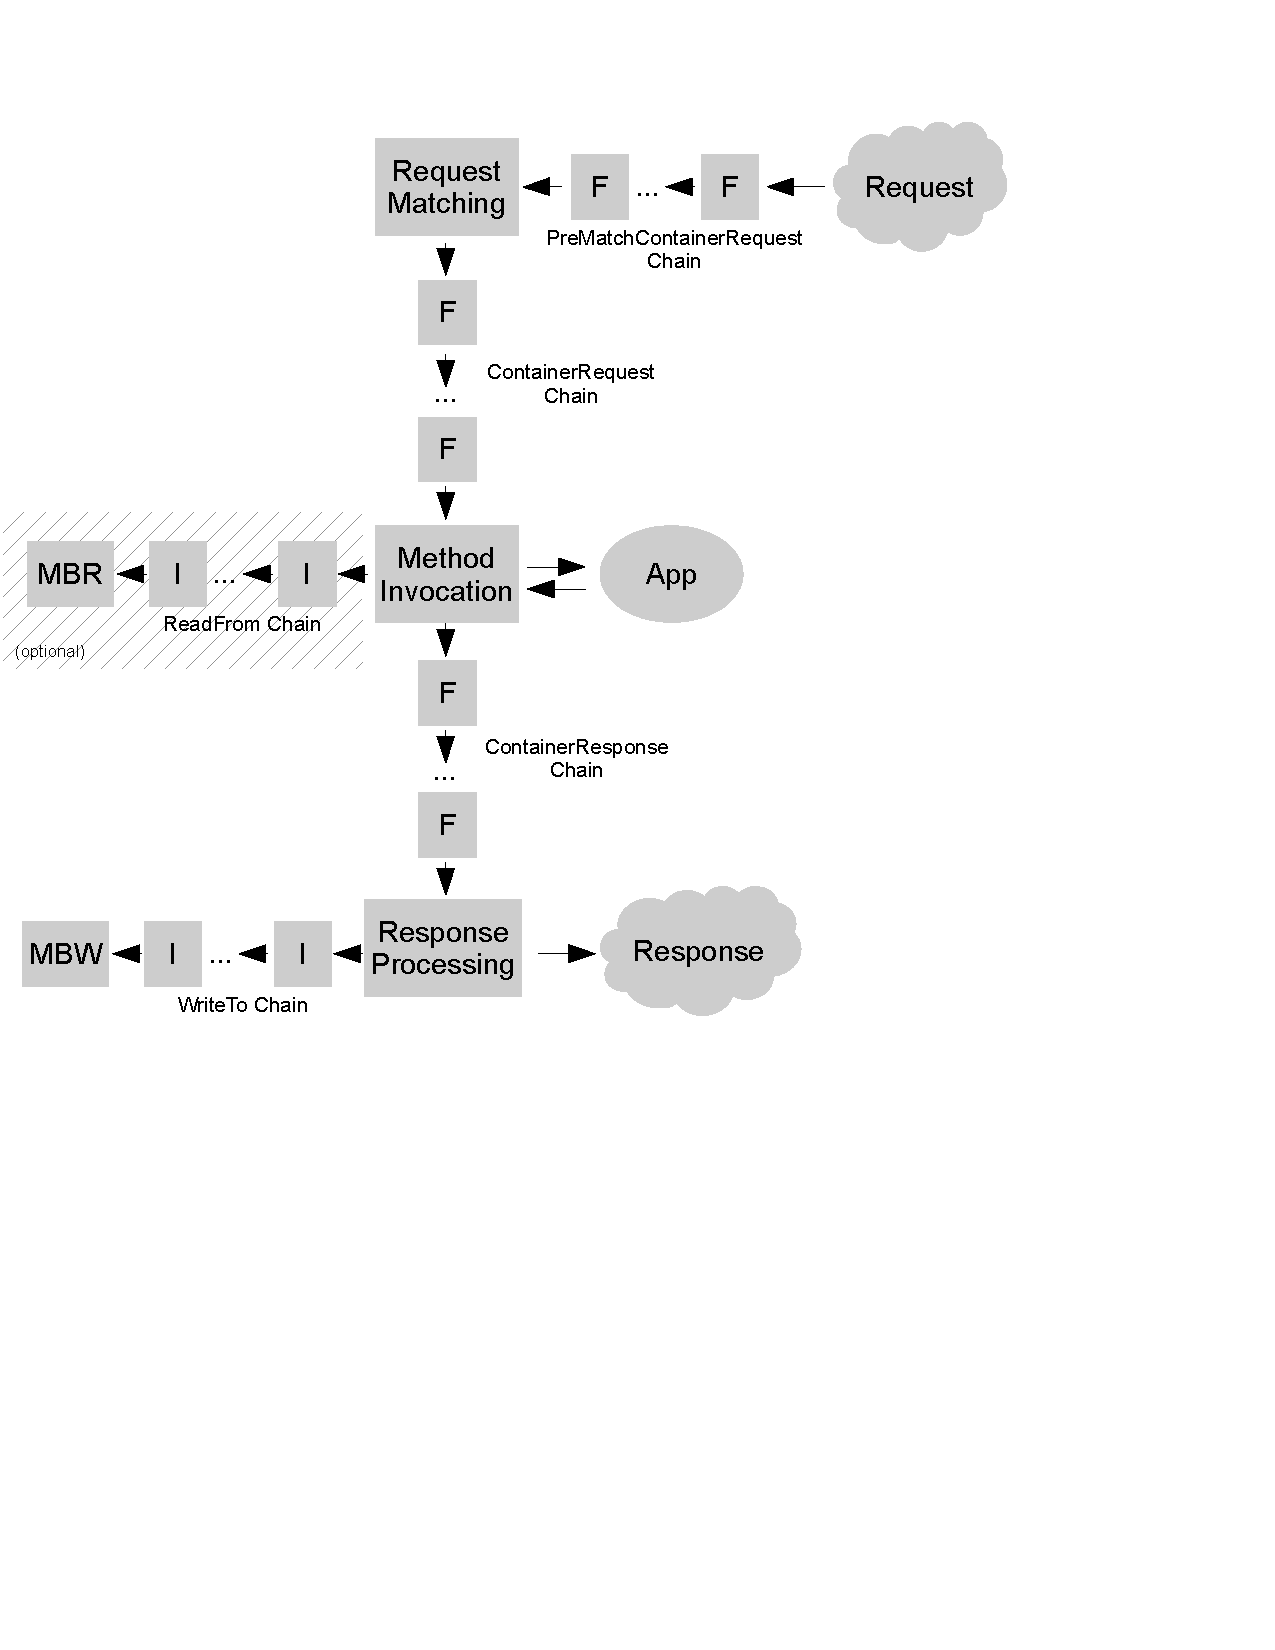
\includegraphics{chapters/pipeline_server.pdf}
\caption{JAX-RS Server Processing Pipeline.}
\end{figure}

\begin{figure}[t]
\label{pipeline_client}
\centering
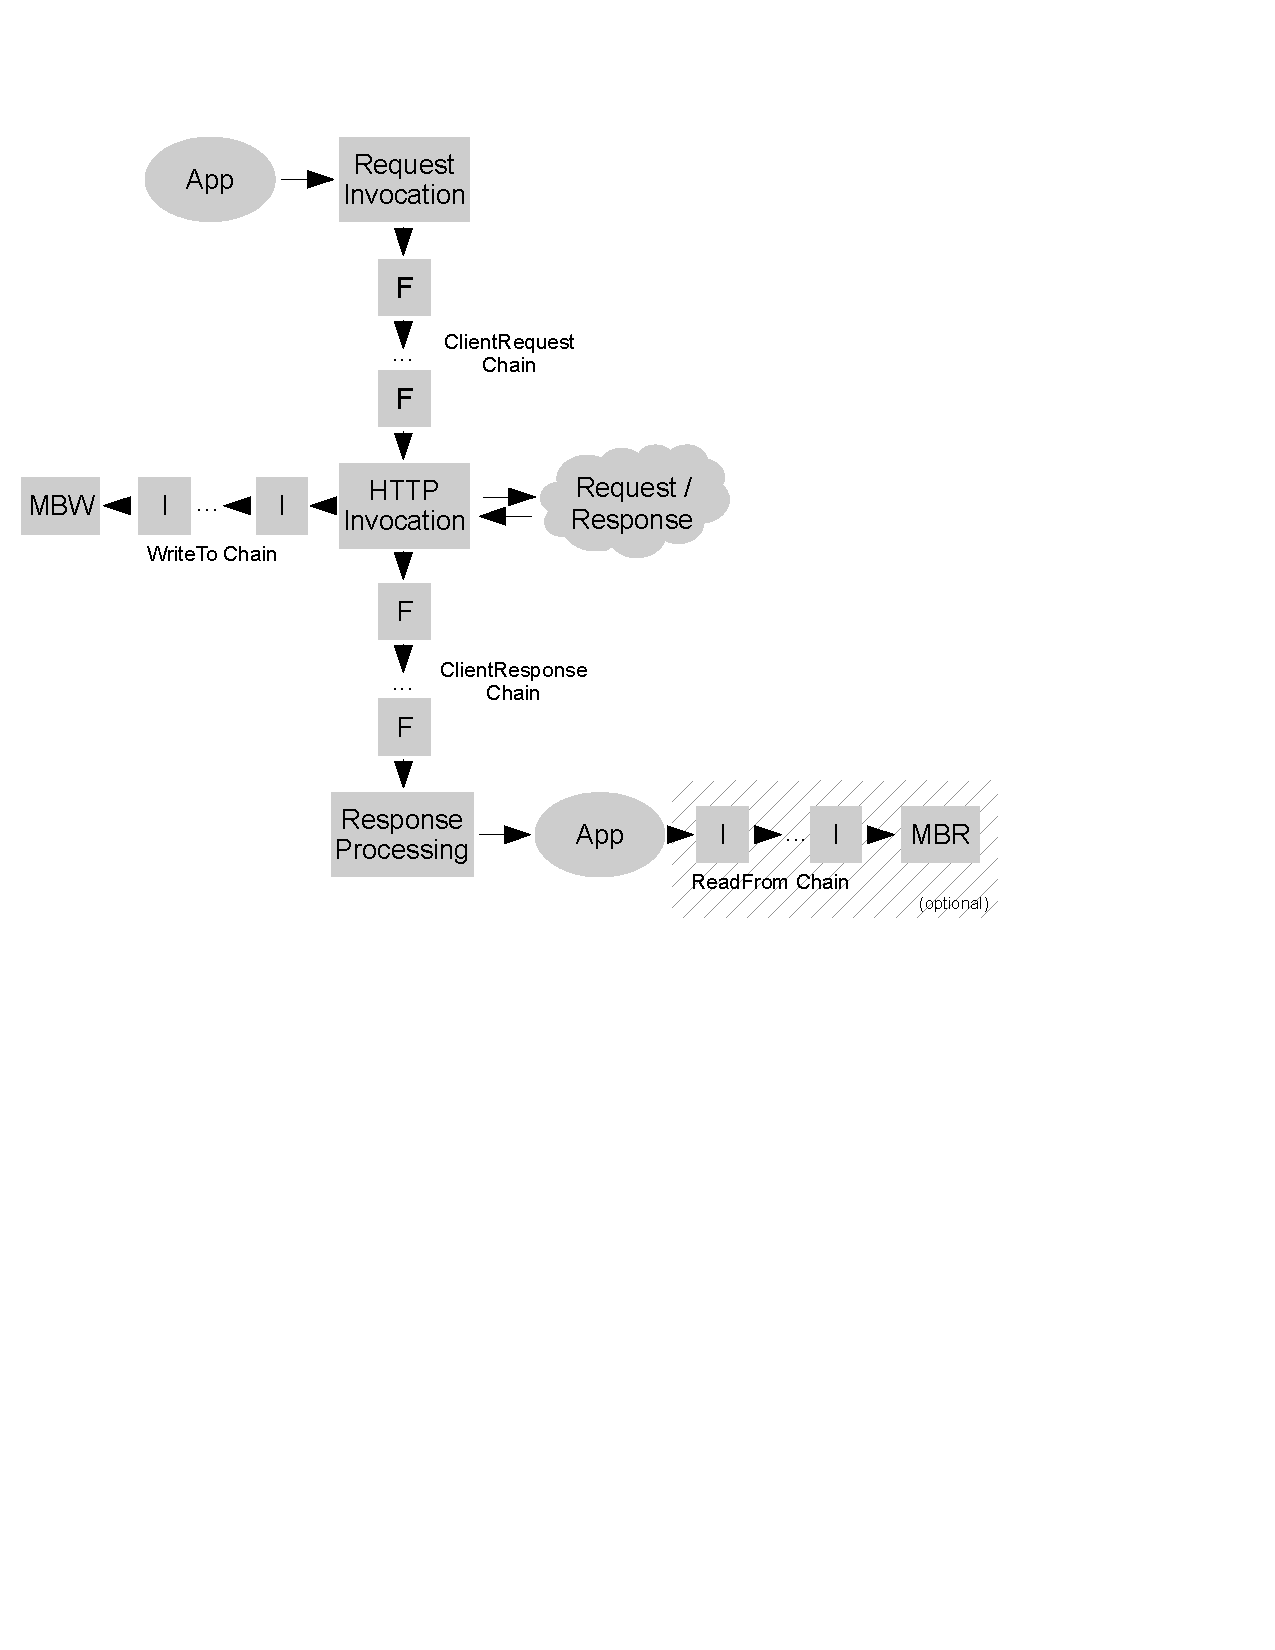
\includegraphics{chapters/pipeline_client.pdf}
\caption{JAX-RS Client Processing Pipeline.}
\end{figure}


\chapter{Change Log}

\section{Changes Since 2.0 Proposed Final Draft}

\begin{itemize}
\item Section \ref{message_body_reader} and \ref{message_body_writer}: Updated last logical step separating client and server runtimes.
\item Section \ref{standard_entity_providers}: New exception \code{NoContentException} to handle zero-length entities. 
\item Section \ref{exceptions_providers} and \ref{exceptions_filters_and_interceptors}: New subsections to separate client and server processing of exceptions.
\item Section \ref{configurable_types}: \Invocation\ and \InvocationBuilder\ are no longer configurable types.
\item Section \ref{filters_interceptors_client}: Updated samples based on changes to Client API.
\item Section \ref{default_validation_mode}: Updated section based on changes to Bean Validation API.
\item Section \ref{validation_and_error_reporting}: Minor re-wording of Phase 2. 
\item Section \ref{timeouts_and_callbacks}: Improved example to return a response if a timeout expires.
\item Section \ref{client_api_async}: Updated samples based on changes to Client API.
\item Section \ref{contexttypes}: Clarified server vs.~client injectable types.
\item Section \ref{configuration_injection}: New section about injection of \code{Configuration} instances.
\item Section \ref{bv_support}: New section stating that support for resource validation is required only in a product that supports Bean Validation.
\end{itemize}

\section{Changes Since 2.0 Public Review Draft}

\begin{itemize}
\item In Javadocs: Method \code{getSize} in class \code{MessageBodyWriter} is deprecated.
\item Chapter \ref{resources} and \ref{providers}: Replaced \WebAppExc\ by corresponding subclass depending on HTTP status code.
\item Section \ref{resource_field}: New step for \code{ParamConverter}. 
\item Section \ref{standard_entity_providers}: Special case for zero-length entities and primitive types.
\item Chapter \ref{client_api}: Updated samples and text related to the configuration of Client API types. Method \code{configuration} has been removed in favor of the \code{Configurable} interface.
\item Chapter \ref{client_api}: \code{ClientFactory} renamed to \code{ClientBuilder}.
\item Chapter \ref{client_api}: Dropped support for \code{@Uri} annotation.
\item Section \ref{entity_interceptors}: New paragraph clarifying that entity interceptors are not called if a \code{readFrom} or \code{writeTo} method is called directly from application code.
\item Section \ref{entity_interceptors}: Improved \code{GzipInterceptor} sample.
\item Section \ref{Name_Binding}: Clarified name binding with multiple annotations. Made semantics compatible with CDI interceptor binding. Name binding with \code{Application} subclasses.
\item Section \ref{priorities}: Annotation \code{@BindingPriority} replaced by common annotation \code{@Priority}.
\item Section \ref{exceptions_filters_and_interceptors}: Clarified processing of a response mapped from an exception.
\item Section \ref{server_api}: Updated samples in this section. New citation for JSR 236.
\item Section \ref{timeouts_and_callbacks}: Improved example.
\item Section \ref{client_api_async}: Fixed signature of method \code{failed} in samples.
\item Section \ref{default_validation_mode}: New section about default validation and \code{@ValidateExecutable}.
\item Section \ref{validation_and_error_reporting}: Restored validation phases.
\item Section \ref{jsonp}: New section about integration with JSON-P.

\end{itemize}

\section{Changes Since 2.0 Early Draft (Third Edition)}

\begin{itemize}
\item Chapter ``Validation'': Removed from PR. JAX-RS 2.0 will defer to CDI for Bean Validation. Only those resource classes that are CDI beans would be validated.
\item Section \ref{method_exc}: Clarified that the steps must be followed in order and that throwables are propagated to the underlying container only if they cannot be mapped.
\item Section \ref{resource_method}: Added \code{@OPTIONS} to list.
\item Section \ref{resource_method_return}: New note about anonymous inner classes.
\item Section \ref{request_matching}: Allow multiple root resource classes to share same URI in algorithm. Note changes in output and input of steps 1 and 2, respectively.
\item Section \ref{message_body_writer}: Throw new exception  \code{InternalServerErrorException}.
\item Section \ref{entity_providers}: Removed steps that required the use of the JavaBeans Activation Framework\cite{jaf} to map objects to representations and vice-versa. The EG deemed this feature to be confusing and not portable across implementations.
\item Section \ref{standard_entity_providers}: Support for pre-packaged readers and writers for Java types \code{java.lang.Boolean}, \code{java.lang.Character}, \code{java.lang.Number} and media type \code{text/plain}.
\item Section \ref{standard_entity_providers}: Detailed behavior for readers and zero-length request entities.
\item Section \ref{dynamic_binding}: \code{DynamicBinder} replaced by \code{DynamicFeature}.
\item Section \ref{exceptions_filters_and_interceptors}: Clarified processing of responses mapped using exception mappers. 
%\item Section \ref{annotations_and_validators}: Explained notion of processing groups and use of \code{Default} group.
\item Chapter \ref{asynchronous_processing}: Updated sections related to the Server API. \code{@Suspended} annotation, timeouts and callbacks.
\item Section \ref{timeouts_and_callbacks}: Throw new exception \code{ServiceUnavailableException}.
\item Section \ref{resource_context}: New section for \code{ResourceContext}.
\item Section \ref{ejbs}: Clarified location of annotations in accordance to the JAX-RS annotation inheritance rules.
\item Chapter \ref{filters_and_interceptors}: Replaced \code{@PostMatching} by \code{@PreMatching}. Post-matching is now the default.
\item Appendix \ref{annotation_table}: Edited section on JAX-RS 2.0 annotations.
\end{itemize}

\section{Changes Since 2.0 Early Draft (Second Edition)}

\begin{itemize}
\item Section \ref{uritemplates}: New example showing a scenario in which a \code{@PathParam} is not be available for injection. 
\item Section \ref{request_matching}: Formalization of certain parts of the matching algorithm that were vague. Defined formal ordering between media types and highlighted situations in which implementations should report a warning if the matching is ambiguous. 
\item Section \ref{request_matching}: New sample showing the resource matching algorithm in action.
\item Section \ref{template_to_regex}: New footnote about syntax of regular expression.
\item Chapter \ref{providers}: The annotation \Provider\ is now only required for automatic discovery of providers (typically via class scanning). It is no longer required for a provider that is manually registered in classes such as \code{Application} or \code{Configuration}.
\item Section \ref{automatic_discovery}: New section about automatic discovery of provider classes. Only those annotated with \Provider\ must be discovered automatically.
\item Chapter \ref{client_api}: Features are now providers and can be registered as such. A feature can no longer be disabled.
\item Chapter \ref{client_api}: Class \code{Target} renamed to \WebTarget. Removed text describing how to use a builder factory class (no longer supported). A few other minor updates and typos fixed.
\item Chapter \ref{filters_and_interceptors}: Extension points for filters revised. New filter interfaces \ClientRequestFilter\ and \ClientResponseFilter\ in Client API and new filter interfaces \ContainerRequestFilter\ and \ContainerResponseFilter\ in Server API. Corresponding context classes also updated in chapter. A \ContainerRequestFilter\ is executed before resource matching unless annotated with \PostMatching. It is no longer possible to share a filter implementation between the Client and Server APIs; entity interceptors are still shareable.
\item Chapter \ref{filters_and_interceptors}: Section on the relationship between filters and entity interceptors (including diagram) dropped.
\item Section \ref{global_binding}: Clarified global binding in relation to the new semantics of \Provider\ for automatic discovery.
\item Section \ref{dynamic_binding}: The \code{DynamicBinding} interface, intended to be implemented by filters and entity interceptors, is replaced by \code{DynamicBinder}. A dynamic binder is a new type of provider that binds filters and entity interceptors with resource methods. 
\item Chapter ``Validation'': Use media type names instead of Java constants for clarity. More descriptive names for constraint annotations. Changed inheritance rules for constraint annotations to follow those defined in \cite{bv11}. New note about \code{@Valid} support for return values. Fixed phase number typo.
\item Section \ref{timeouts_and_callbacks}: New sentence about calling \code{suspend} more than once or in a method annotated with \code{@Suspend}.
\item Section \ref{async_ejbs}: New section about EJB resource classes with methods annotated with \code{@Asynchronous}.
\item Chapter \ref{environment}: Re-structured chapter with sub-sections for each of the EE technologies with which \jaxrs\ integrates. New examples added.
\end{itemize}

\section{Changes Since 2.0 Early Draft}

\begin{itemize}
\item Section \ref{expert_group}: Updated 2.0 expert group member list.
\item Section \ref{acks}: Updated acknowledgements for 2.0 version.
\item Section \ref{exceptions_providers}: New section that describes exception handling for all providers. Related changes to reference this new section.
\item Section \ref{exceptions_filters_and_interceptors}: New section for filter and interceptor exceptions. Related changes to reference this new section.
\item Section \ref{request_matching}: Updated step 2a so that it only goes to step 3 when $M \neq \{\}$. 
\item Section \ref{request_matching}: New sentence about the use of a server quality parameter (qs-value) during request matching.
\item Chapter \ref{filters_and_interceptors}: New extension point for pre-match filters that are executed before resource matching.
\item Chapter \ref{filters_and_interceptors}: Filter methods no longer return a next action; the execution of a request filter chain is stopped by setting a response in the associated context.
\item Chapter \ref{filters_and_interceptors}: Handlers renamed to entity interceptors for clarity (in this log included).
\item Section \ref{global_binding}: Global binding is now the default for filters and entity interceptors. The annotation \code{@GlobalBinding} has been dropped.
\item Section \ref{priorities}: Clarified reverse ordering of the response filter chain based on binding priorities.
\item Appendix C: Removed from this version after changes to Chapter \ref{filters_and_interceptors}.
\item Chapter ``Validation'': Moved to an instantiate-then-validate strategy in which validation of constructor parameters and setters is no longer supported. Simplified validation process to better align with Bean Validation 1.1 \cite{bv11}. In particular, validation of resource classes, fields and property getters are all carried out in a single step.

\end{itemize}

\section{Changes Since 1.1 Release}

\begin{itemize}
\item Section \ref{status}: Updated URLs to JSR pages, etc.
\item Section \ref{non_goals}: Removed Client APIs as non-goal.
\item Section \ref{terminology}: Added new terminology.
\item Section \ref{expert_group}: List 2.0 expert group members.
\item Section \ref{acks}: acknowledgements for 2.0 version.
\item Chapter \ref{applications}: Somewhat generic section on validation removed to avoid confusion with the type of validation defined in Chapter ``Validation''.
\item Section \ref{servlet}: Clarified used of Servlet 3 framework pluggability. Added sample web.xml files and a table summarizing all cases.
\item Section \ref{entity_parameters}: Clarified notion of entity parameter as a parameter not annotated with any JAX-RS annotation.
\item Section \ref{declaring_method_capabilities}: Explained use of quality factor q. Introduced server-side quality factor qs and included example.
\item Section \ref{annotationinheritance}: Added sentence about conflicting annotations and recommendation to repeat annotations for consistency with other Java EE specifications.
\item Section \ref{reqpreproc}: Highlighted input and output for each step in algorithm. Minor edits to simplify presentation.
\item Section \ref{determine_response_type}: Updated algorithm to support server-side quality factor qs.
\item Chapter \ref{client_api}: New chapter Client API.
\item Chapter \ref{filters_and_interceptors}: New chapter Filters and Interceptors.
\item Chapter ``Validation'': New chapter Validation.
\item Chapter \ref{asynchronous_processing}: New chapter Asynchronous Processing.
\item Appendix \ref{annotation_table}: New section for 2.0 annotations.
\item Appendix C: New appendix describing filter and interceptor extension points.
\end{itemize}

\section{Changes Since 1.0 Release}

\begin{itemize}
\item Section \ref{servlet}: New requirements for Servlet 3 containers.
\item Section \ref{javaee}: Requirements for Java EE 6 containers.
\item Section \ref{standard_entity_providers}: Requirements on standard entity providers when presented with an empty message entity.
\item Section \ref{message_body_writer}: Add closeness of generic type as secondary sort key.
\item Section \ref{message_body_reader}: Default to application/octet-stream if a request does not contain a content-type header.
\item Section \ref{resource_field}: Add support for static fromString method.
\item Section \ref{annotationinheritance}: Clarify annotation inheritance.
\item Section \ref{security_context}: Fix typo.
\item Section \ref{servlet_container}: Additional considerations related to filters consuming request bodies.
\end{itemize}

\section{Changes Since Proposed Final Draft}

\begin{itemize}
\item Section \ref{request_matching}: Additional sort criteria so that templates with explicit regexs are sorted ahead of those with the default.
\item Sections \ref{request_matching}, \ref{determine_response_type}, \ref{declaring_provider_capabilities} and \ref{context_media_type}: Q-values not used in \Consumes\ or \Produces.
\item Section \ref{message_body_writer}: Fixed algorithm to refer to Section \ref{determine_response_type} instead of restating it. Fixed status code returned when the media type has been determined but an appropriate message body writer cannot be located.
\item Chapter \ref{runtimedelegate}: Clarify that an implementation can supply an alternate \rd\ API class.
\end{itemize}

\section{Changes Since Public Review Draft}

\begin{itemize}
\item Chapter \ref{applications}: Renamed ApplicationConfig class to Application.
\item Chapter \ref{resources}: UriBuilder reworked to always encode components.
\item Sections \ref{resource_class_constructor} and \ref{provider_class_constructor}: Added requirement to warn when choice of constructor is ambiguous.
\item Section \ref{resource_field}: \code{FormParam} no longer required to be supported on fields or properties.
\item Section \ref{resource_method_return}: Added text describing how to determine raw and generic types from method return type and returned instance.
\item Section \ref{uritemplates}: Template parameters can specify the regular expression that forms their capturing group.
\item Section \ref{reqpreproc}: Make pre-processed URIs available rather than original request URI. Added URI normalization.
\item Section \ref{reqpreproc}: Removed URI-based content negotiation.
\item Section \ref{request_matching}: Reorganized the request matching algorithm to remove redundancy and improve readability, no functional change.
\item Section \ref{template_to_regex}: Changes to regular expressions to eliminate edge cases.
\item Section \ref{entity_providers}: Added requirement to use JavaBean Activation Framework when no entity provider can be found.
\item Section \ref{standard_entity_providers}: Require standard JAXB entity providers to use application-supplied JAXB contexts in preference to their own.
\item Section \ref{contextprovider}: Added support for specifying media type capabilities of context providers.
\item Section \ref{contexttypes}: Removed \code{ContextResolver} from list of injectable resources.
\item Section \ref{providercontext}: Changed name to Providers, removed entity provider-specific text to reflect more generic capabilities.
\item Chapter \ref{headersupport}: New appendix describing where particular HTTP headers are supported.
\end{itemize}


\backmatter

\raggedright
\bibliographystyle{unsrt}
\addcontentsline{toc}{chapter}{Bibliography}
\bibliography{references}



\end{document}
